\documentclass[10pt,a4paper]{article}

\usepackage{amsmath}

\usepackage{inputenc}
\usepackage{fvextra}

\usepackage{algpseudocode}
\usepackage{algorithmicx}
\usepackage{amsfonts}
\usepackage{amssymb}
\usepackage{amsthm}
\usepackage[spanish]{babel}
\usepackage{bm}
\usepackage{booktabs} % To thicken table lines
\usepackage{bussproofs}
\usepackage{caption}
\usepackage{csquotes}
\usepackage{colortbl}
\usepackage{dsfont}
\usepackage{environ}
\usepackage[shortlabels]{enumitem}
\usepackage{fancyhdr}
\usepackage{forest}
\usepackage{geometry}
\usepackage{graphicx}
\usepackage[hidelinks]{hyperref}
\usepackage{ifthen}
\usepackage{multicol}
\usepackage{multirow}
\usepackage{sidecap}
\usepackage{stmaryrd}
\usepackage{tabularx}
\usepackage{titling}
\usepackage{tikz}
\usepackage{xcolor}
\usepackage{wrapfig}
\usepackage{minted}

\usetikzlibrary{arrows}
\usetikzlibrary{arrows.meta}
\usetikzlibrary{automata}
\usetikzlibrary{calc}
\usetikzlibrary{fit}
\usetikzlibrary{matrix}
\usetikzlibrary{positioning}
\usetikzlibrary{shapes.geometric}
\usetikzlibrary{shapes.multipart}

\newcommand{\red}[1]{{\color{red}#1}}
\newcommand{\green}[1]{{\color{green}#1}}
\newcommand{\blue}[1]{{\color{blue}#1}}
\newcommand{\violet}[1]{{\color{violet}#1}}
\newcommand{\orange}[1]{{\color{orange}#1}}

\newcommand{\nat}{\mathbb{N}}
\newcommand{\reales}{\mathbb{R}}

\newtheorem{theorem}{Teorema}
\newtheorem{coro}{Corolario}
\newtheorem{proposicion}{Proposición}
\newtheorem{lema}{Lema}


\usetikzlibrary{shapes.multipart}

\tikzstyle{demoBox} = [
draw=blue!20, very thick,
rectangle split, rectangle split parts=2, rounded corners, inner xsep=0.5cm,
rectangle split part fill = {blue!20, blue!5}
]

\tikzstyle{demoPart} = [
draw=blue!20, very thick,
rounded corners, inner xsep=0.5cm,
fill = blue!5
]
%\newcommand{\qed}{\begin{flushright}
%		$\blacksquare$
%\end{flushright}}

\NewEnviron{demo}[1][]{%
	\begin{center}
		\begin{tikzpicture}
			\node [demoBox](box){%
				\textbf{\scriptsize
					DEMOSTRACIÓN #1}
				\nodepart{two}
				\begin{minipage}{0.75\textwidth}
					\vspace*{0.1cm}
					\BODY
				\end{minipage}
			};
		\end{tikzpicture}
	\end{center}
}

\NewEnviron{demoPart}[1][]{%
	\begin{center}
		\begin{tikzpicture}
			\node [demoPart](box){%
				\begin{minipage}{0.75\textwidth}
					\vspace*{0.1cm}
					\BODY
				\end{minipage}
			};
		\end{tikzpicture}
	\end{center}
}


\title{Sistemas Operativos - Apuntes para final}
\author{Gianfranco Zamboni}

\usemintedstyle[cpp]{bordeland, tabsize=2}
%%%% CONFIGURACIONES %%%%

%% La coma de los reales es un punto
\decimalpoint{}

%%% Tamaño de pagina
%\geometry{
%	includeheadfoot,
%	left=2.54cm,
%	bottom=1cm,
%	top=1cm,
%	right=2.54cm
%}

%\stul{0.1cm}{0.2ex}

%% HEADER Y FOOTER
\pagestyle{fancy}

\fancyhf{}

\fancyhead[LO]{\rightmark} % \thesection\ 
\fancyhead[RO]{\small{\thetitle}}
\fancyfoot[CO]{\thepage}
\renewcommand{\headrulewidth}{0.5pt}
\renewcommand{\footrulewidth}{0.5pt}
\setlength{\headsep}{1cm}
\setlength{\headheight}{13.07225pt}

\renewcommand{\baselinestretch}{1.2}  % line spacing

%% Links en indice 
\hypersetup{
	linktoc=all,     %set to all if you want both sections and subsections linked
	linkcolor=blue,  %choose some color if you want links to stand out
}
\setcounter{tocdepth}{2}
\begin{document}

	\maketitle
	\tableofcontents

\newpage
\section{Introducción}
\subsection{La semilla del internet}  
El telégrafo fue el antecesor del teléfono, un primer acercamiento a la comunicación de
mensajes vía una codificación. Desde fines de siglo XIX hasta segunda mitad del siglo XX,
aparecen las centrales de \textbf{conmutación de circuitos} (centrales telefónicas). A estas centrales
llegaban señales (cables) correspondientes a todas las casas que participacen en el sistema de
teléfonos. Las operadoras conectaban dos circuitos en sus tableros para cerrar el circuito y
permitir la comunicación entre las dos partes involucradas. Sin embargo, este tipo de comunicación tenía una gran falla: Si una central de conmutación de circuitos
dejaba de estar disponible por algún motivo de fuerza, todas las personas pertenecientes a esa
zona se verían incomunicadas.


A fines de los 50 se empieza a desarrollar la \textbf{conmutación de paquetes} buscando resolver este tema, es decir se busca una \textbf{red más tolerante a fallas}, \textbf{más flexible} a la hora de conectar dos puntos distantes y que \textbf{escale más facilmente} ante un incremento en el acceso a la comunicación.

La nueva red propuesta es una red descentralizada con mútiples caminos entre dos puntos que divide los paquetes en fragmentos que pueden llegar a destino a través de distintos caminos.

\subsection*{El modelo OSI}
En 1983 aparece una publicación de ISO para establecer un estándar que especifique la estructura de una arquitectura de red, que uniformice la forma de construir las redes de cominucación: el modelo OSI-ISO (Open Systems Interconnection).

\begin{figure}[h]
	\centering
	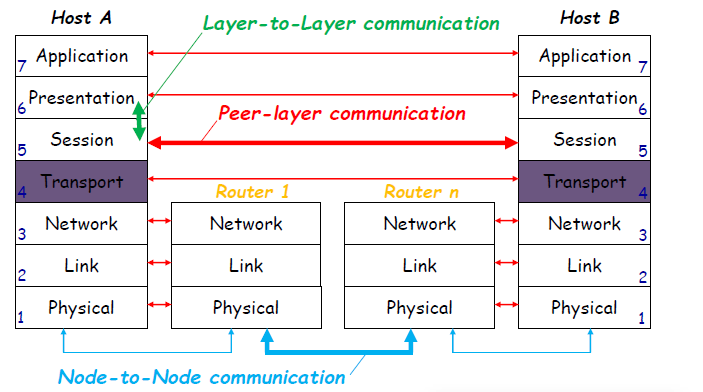
\includegraphics[width=0.65\textwidth
]{images/osi.png}
	\caption[Modelo OSI de Referencia]{Modelo OSI}
	\label{fig:osi}
\end{figure}

Este modelo está dividido en 7 capas, cada una de las cuales tiene una función definida que permitirán la comunicación coherente entre dos sistemas remotos.  

\begin{enumerate}
  \item La capa \textbf{física (Physical)} se encarga de enviar raw bits a través de los medios físicos disponibles en la red. 
  \item La capa de \textbf{enlace (Link)} se encarga de detectar errores en la transmisión y corregirlos, si es posible.
  \item La capa de \textbf{red (Network)} se encarga de resolver problemas de congestión dentro de la red, que paquetes se aceptan y la ruta que deben tomar los paquetes que se envían por la misma.
  \item La capa de \textbf{transporte (Transport)} se encarga de tomar la información provista por la capa de arriba, pasarla a la capa de red separada en pedazos más chicos (\textbf{chunks}) y se asegura que todas las partes lleguen a destino correctamente. 
  
  Esta es la primer capa \textbf{end-to-end}, es decir que entabla una ``conversación'' entre la máquina emisora (\textbf{Source}) y la destinataria (\textbf{Destination}). Las capas anteriores, usan protocolos de comunicación nodo a nodo, es decir, entre una máquina y su vecino inmediato y no entre el source y el destination que podrían estar separados entre sí por varios nodos.
  
  \item La capa de \textbf{sesión  (Session)} permite establecer sesiones entre dos máquinas distintas. Estas sesiones permiten sincronizar el pasaje de información entre ambas máquinas, deciden de quien es el turno para enviar información y evitar que ambas máquinas realizen operaciones críticas de manera simultanea.
  \item La capa de \textbf{presentación (Presentation)} procesa la información recibida, la estructura y la codifica de la manera necesaria para que pueda ser usada por la máquina.
  \item La capa de \textbf{aplicaciones (Application)} contiene los protocolos necesarios para que los usuarios puedan ver y leer la información.
\end{enumerate}

Además de estas funcionalidades, cada capa ofrece una interfaz que le permite comunicarse con las capas vecinas para hacer el pasaje de los datos entre ellas y asumen que el host en el otro extremo de la comunicación tendrá una arquitectura similar y podrá interpretar los mensajes de cada una de ellas.

\subsection{Modelo TCP/IP}
\begin{figure}[H]
	\centering
	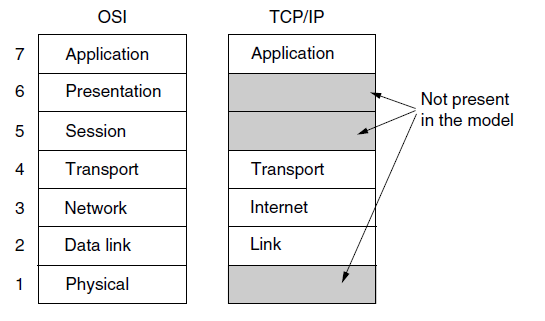
\includegraphics[width=0.65\textwidth
]{images/tcpip.png}
	\caption[Modelo TCP/IP de Referencia]{Modelo TCP/IP}
	\label{fig:tcp}
\end{figure}

Fue diseñado con el objetivo de mantener las conexiones intactas mientras ambos puntos finales de conexión estén funcionando, incluso si laguno de las máquinas o líneas entre ellos fuese dado de baja.

\begin{enumerate}
  \item La capa de \textbf{enlace (Link)} maneja la infraestructura física de la red y permite que dos nodos se puedan comunicar entre si. Se encarga de convertir los bits enviados por la capa superior a señales analógicas y transmitirlas a través de los medios físicos disponibles.
  \item La capa de \textbf{intrared (internet)} permite al host injectar paquetes en cualquier red y se encarga de hacerlos llegar a destino. Esto se hace de manera independiente para cada paquete, es decir pueden no seguir el mismo camino e incluso podrían llegar en distinto orden. En el último caso corresponde a la capas superiores reodenarlos para que puedan ser procesados, si es necesario.
  \item La capa de \textbf{transporte (Transport)} debe ser diseñada para permitir que dos entidades de la red puedan mantener una conversación. Aquí se definieron dos protocolos:
  \begin{itemize}
    \item El \textbf{Transmission Control Protocol (TCP)} que permite enviar sin errores un stream de bytes desde una máquina a otra en la red.
    \item El \textbf{User Datagram Protocol (UDP)} que permite evitar todo el flujo de conexión TCP y crear el suyo propio. En general, se usa en aplicaciones que requieren una respuesta más rápida que precisa. 
  \end{itemize}
  \item La capa de \textbf{Aplicación (Application)} es en la que se incluyen la sesiones y funciones necesarias para codificar y procesar los paquetes enviados y recibidos. Entre los protocolos usados en esta capa se encuentran: TELNET, FTP y SMTP.
\end{enumerate}


\newpage
\part{Nível Físico}
\section{Teoría de la información}
\subsection{Información}
Sea \(E\) un suceso que puede presentarse con probabilidad \(P(E)\). Cuando \(E\) tiene lugar, decimos que hemos recibido \[I(E)=\log\frac
{1}{P(E)}\] unidades de información.

Si introducimos el logaritmo de base 2, la unidad se denomina \textit{bit}. Notemos, también, que si \(P(E) = \frac{1}{2}\), \(I(E) = 1\) bit. Es decir, un bit es la cantidad de información obtenida al especificar una de dos posbiles alternativas igualmente probables.

\subsubsection{Fuentes de Memoria Nula}
Son fuentes de información que emiten una secuencia de símbolos pertenecientes a un alfabeto finito y fijo \(S=\{s_1,\dots,s_n\}\) de manera estadísticamente independientes. Estas fuentes pueden describirse mediante el alfabeto \(S\) y las probabilidades con que los simbolos se presentan: \(P(s_1), \dots, P(s_n)\).

La información que aporta cada símbolo de la fuente \[I(s_i) = \log_2\frac{1}{P(s_i)}\text{ bits}\]
\subsubsection{Entropía}
Dada una fuente de memoria nula \(S\) con alfabeto \({s_1,\dots,s_n}\), la entropía \(H(S)\) es la cantidad media de información por símbolo de la fuente, es decir:
\[H(S) = \sum_{i=1}^n P(s_i)I(s_i) = \sum_{i=1}^n P(s_i)\log_2\frac{1}{P(s_i)} = -\sum_{i=1}^n P(s_i)\log_2 P(s_i)\text{ bits} \]

Podemos interpretar la entropía como el \textbf{valor medio ponderado de la cantidad de información} del conjunto de mensajes posibles, como una medida de la \textbf{incertidumbre probmedio (grado de incerteza)}acerca de una variable aleatoria o la \textbf{cantidad de información} obtenida al observar la aparición de cada nuevo símbolo.

\paragraph{Propiedades:}
\begin{itemize}
  \item La entropía es no negativa y se anula si y solo si la probabilidad de uno de sus símbolos es 1 y la del resto es 0.
  \item La entropía máxima (\textbf{mayor incertidubme del mensaje}) se logra cuando todos los símbolos que puede ser emitidos por la fuente son equiprobables.
    \item Si hay \(n\) símbolos equiprobables \(P(s)=\frac{1}{n}\) se cumple:
    \[
      H(S) = -\sum_s P(S)\log_2 P(S) = -n(\frac{1}{n}\log_2\frac{1}{n}) = -(\log_2 1 - log_2 n) = \log_2 n
    \]
\end{itemize}

\subsubsection{Extensión de memoria nula}
Si tenemos una fuente de memoria nula \(S\), con un alfabeto \(\{s_1,\dots,s_q\}\), podemos agrupar las salidas en paquetes de \(n\) símbolos. Tendremos, pues, \(qn\) secuencias de salidas distintas. 

Formalmente, sea \(S\) una fuente de información de memoria nula con un alfabeto \(\{s_1,\dots,s_q\}\). Sea \(P_i\) la probabilidad correspondiente a \(s_i\). Entonces, la extensión de orden \(n\) de \(S\) \((S^n)\) es una fuente de memoria nula de \(qn\) símbolos \(\{\sigma_1,\dots,\sigma_{qn}\}\) donde cada \(\sigma_i\) corresponde a una secuencia de simbolos de \(S\) de longitud \(n\). La probabilidad de \(\sigma_i\), \(P_{\sigma_i}\) es la probabilidad de la secuencia correspondiente. Es decir, si \(\sigma = s_{i_1}\dots s_{i_k}\) entonces \(P(\sigma) = P_{i_1}\dots P_{i_k}\).

Puesto que un símbolo de \(S^n\) corresponde a \(n\) símbolos de \(S\), es de suponer que la entropía por símbolo de \(S^n\) sea \(n\) veces mayor que la de \(S\), osea:
\[H(S^n) = nH(S)\]

\subsection{Codificación}
Sea \(S = \{ s_1,\dots, s_q\} \) el conjunto de símbolos de un alfabeto dado. Se define un \textbf{código} como la correspondencia de todas las secuencias posibles de símbolos de \(S\) a secuencias de símbolos de algún otro alfabeto \(X =\{x_1,\dots x_r\}\). \(S\) recibe el nombre de \textbf{alfabeto fuente} y \(X\) el de \textbf{alfabeto código}.

Cuando codificamos un alfabeto fuente, buscamos lograr una representación eficiente de la información mediante la eliminación de la redundancia.q

\paragraph{Código bloque:} Es aquel que asigna cada uno de los símbolos del alfabeto fuente \(S\) a una secuencia fija de símbolos del alfabeto código \(X\). Esas secuencias fijas (secuencias de \(x_i\)) reciben el nombre de palabras
código. Denominaremos \(X_i\), a la palabra código que corresponde al símbolo \(s_i\).

\paragraph{Código no singular:} Es un código en el que todas sus palabras son distintas.

\paragraph{Extensión de orden n:} La extensión \(C^n\) de orden \(n\) de un código bloque \(C:S\to X^*\), es el código bloque que hace corresponder las secuencias de símbolos de \(S\) con las secuencias de las palabras código formadas por \(C(s_i)\). Es decir: Si \(s_i\dots s_k\in S^*\), entonces \(C^n(s_i\dots s_k) = C(s_i)\dots C(s_k)\).

\paragraph{Código univócamente decodificable:} Es aquel en el cual ninguna tira de símbolos del alfabeto código admite más de una única decodificación. Dicho de otra forma, un código bloque se dice univocamente decodificable si, y solamente si, su extensión de orden \(n\) es no singular para, cualquier valor finito de \(n\).

\paragraph{Código instantaneo:} Un código unívocamente decodificable se denomina instantáneo cuando es posible decodificar las palabras de una secuencia sin precisar el conocimiento de los símbolos que las suceden.

\paragraph{Préfijo de una palabra:} Sea \(X=x_1\dots x_m\) una palabra de un código. Se denomina prefijo de esta palabra a la secuencia de símbolos \(x_1\dots x_j\), donde \(j \leq m\).

La condición necesaria y suficiente para que un código sea instantáneo es que ninguna palabra del código coincida con el prefijo de otra.

\paragraph{Inecuación de Kraft:} Dado un alfabeto \(S = \{s_1,\dots,s_n\}\) y un alfabeto de código \(X=\{x_1,\dots,x_m\}\), es condición necesaria y suficiente, para exista un código instantáneo con palabras de longitud \(l_1,\dots,l_{n}\), que se cumpla la siguiente inecuación:
\[\sum_{i=1}^n |X|^{-l_1}\leq 1\]

\subsubsection{Codificación óptima}
Buscamos codificar un alfabeto \(S\) de tal forma que máximizar la relación entre la entropía \(H(S)\) y la longitud media del código \(L\).  Sea \(l_i\) la longitud de la palabra que codifica al símbolo \(s_i\) de la fuente, \(p_i\) la probabilidad de aparicion de \(s_i\) y \(r\) la cantidad de símbolos diferentes en el alfabeto del código entonces:

\begin{itemize}
  \item \(L = \sum p_iL_i \) es la longitud medía del código.
  \item \(\log r\) es la cantidad promedio máxima de información de un símbolo del código.
  \item \(h = \frac{H(S)}{L\log r}\) es la eficencia del código.
\end{itemize}

La máxima eficencia se logra cuando \(h = 1\). En general, esto sucede cuando se asigna las palabras de código más cortas a los símbolos de fuente más probables. También se puede deducir: \[1 \geq h \geq \frac{H(S)}{L\log r}\Rightarrow L\log r \geq H(S)\]

\paragraph{Primer teorema de Shannon (Teorema de la codificación sin ruido):} Sea \(S\) una fuente de memoria no nula, y \(S^n\) la extensión de orden \(n\) de \(S\).  Sea \(C:S^n\to X^n\) un código y \(L_n\) la longitud media de los códigos correspondientes a los símbolos de \(S^n\):
\[
    L_n = \sum_{\sigma\in S^n} C(\sigma)P(\sigma)
\]
Entones vale:
\[
    H(S) \leq \frac{L_n}{n} \leq H(S) + \frac{1}{n}
\]

Esto nos dice que el número medio de símbolos de \(C\) correspendientes a un símbolo de la fuente puede hacerse tan pequeño (pero no inferior) como la entropía de la fuente. El precio que se paga por la disminución de \(L_n\) es un aumento en la complejidad de la codificación debido al gran número de símbolos de la fuente que hay que manejar.

En particular:
\[
  H(S) = \sum_{\sigma\in S^n} C(\sigma)P(\sigma)  
\]

\paragraph{Codificador óptimo:} Es un codificador que usa la menor cantidad posible de bits para codificar un mensaje, es decir: Un codificador se dice óptimo si no existe ningún código para la misma fuente con menor longitud media.

Sea \(s_i\in S\), entonces la cantidad de bits necestarios para representarlo en un codificador óptimo es \(\lceil\frac{1}{P(s)}\rceil\) y la entropía de \[H(X) = \sum_{s\in S} P(s)\log_2\left(\frac{1}{P(s)}\right)\]

\paragraph{Codificación de Huffman:} Es una forma de definir códigos óptimos asumiendo que se conoce la probabilidad de ocurrencia de los símbolos, que la codificación es símbolo por símbolo y la probabilidad de ocurrencia de cada símbolo es independiente.

Dado un mensaje \(M\):
\begin{enumerate}
  \item Se extrae del mismo la frecuencia de cada símbolo.
  \item Se ordenan los símbolos en arbol dependiendo de la frecuencia de cada uno. Mientras más cerca de la raíz, más frecuente es el símbolo.
  \item El código de un símbolo será entonces el camino de la raíz al nodo donde está ubicado (utilizando
  ceros cuando se toma la rama izquierda y 1 cuando se toma la rama derecha).
\end{enumerate} 

Así, los símbolos más frecuentes tendrán los códigos más cortos.





\newpage
\section{Señales}
\subsection{Fundamentos de las señales}
Las señales que se envían por el canal físico para comunicar dos extremos de un canal son \textbf{ondas electromagnéticas} que se propagan a través del canal a una cierta velocidad determinada por el tipo de canal que estemos usando.


Podemos definir todas las señales con una función períodica \(f(t)\) llamada \textbf{frecuencia}. Esto significa que \(f(t) = f(t + T)\) para alguna constante \(T\). Al minimo valor positivo mayo que cero de \(T\) que cumple esto, lo llamamos \textbf{período fundamental}. \(f\) se mide en Hertz o ciclos por segundo y \(T\) en segundos. 

En base a a la frecuncia y el período de una onda definimos:

\begin{itemize}
  \item \textbf{Amplitud:} Indica la cantidad de cambios en la presión del aire. Se mide en decibeles (db o volts). Por decirlo de otra forma, la amplitud es la distancia entre el eje horizontal y el punto más alto del pico de la onda, o el punto más bajo de la depresión de la onda.
  \item \textbf{Frecuencia angular:} \(\omega = 2\pi f\) radianes por segundos.
  \item \textbf{Fase:} \(\phi\): Compara el tiempo entre dos ondas y se mide en grados, de 0 a 360. Cuando dos ondas comienzan al mismo tiempo, se dice que están en fase o alineadas en fase. Cuando una onda se encuentra ligeramente retrasada en comparación con otra onda, se dice que las ondas están desfasadas.
  \item \textbf{Longitud de onda:} Es la distancia entre los ciclos repetitivos de una onda a una frecuencia dada. Cuanto más elevada sea la frecuencia, más corta será la longitud de onda: \[\lambda = \frac{c}{f}\]
  donde \(c=3*10^8\frac{m}{s}\) es la velocidad de la luz.
\end{itemize}
\begin{figure}[H]
	\centering
	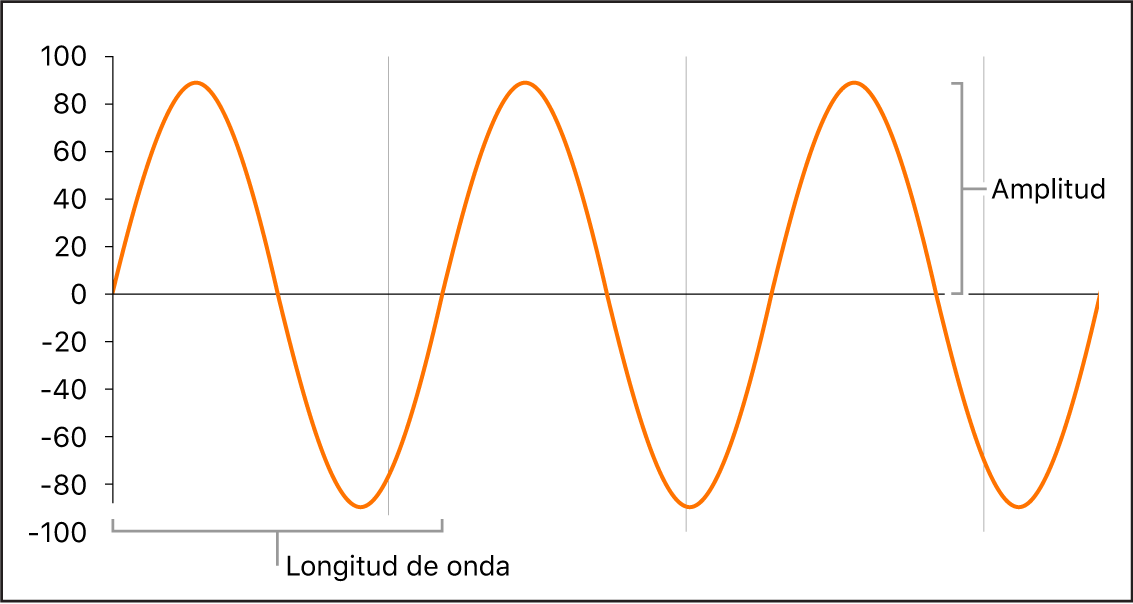
\includegraphics[width=0.65\textwidth
]{images/amplitud.png}
	\caption[Onda de señal]{Onda de señal}
	\label{fig:sistema-comunicacion-real}
\end{figure}

Esta onda puede chocar con imperfecciones del material (del canal), producir reflexiones y refracciones que se traducen en \textbf{perdidas} (menos energía para la señal original en la que está codificado el mensaje)

Dado que las ondas electromagnéticas son continuas y que son modificadas a medida que se propagan por el canal, debemos encontrar una manera de mapear estas frecuencias a los 0 y 1 que componen nuestros mensajes.

Para esto, tanto el transmisor como el recibidor definen un \textbf{ancho de banda} que es el rango de frecuencias que va a ocupar las señales que van a ser transmitidas por el canal y dentro de ese rango, cuales deben ser mapeadas a un 1 y cuales a un 0.

\subsection{Transformación de fourier}
Todas las funciones períodicas pueden expresarse como una suma infinita de senos y cosenos:

\[f(t) = \frac{1}{2}c + \sum_{i=0}^\infty \left(a_i\sen(n\omega t) + b_i\cos(n\omega t)\right)\]

done \(\omega\) es la frecuencia angular y \(a_i\) es la amplitdud de la onda.

Ninguna instalación transmisora puede transmitir señales sin perder cierta potencia en el proceso. Si todos los componentes de Fourier disminuyeran en la misma proporción, la señal resultante se reduciría en amplitud, pero no se distorsionaría. Desgraciadamente, todas las instalaciones de transmisión disminuyen los distintos componentes de Fourier en diferente grado, lo que provoca distorsión. Por lo general, las amplitudes se transmiten sin ninguna disminución desde 0 hasta cierta frecuencia \(f_c\) y todas las frecuencias que se encuentren por arriba de esta frecuencia de corte serán atenuadas. El rango de frecuencias que se transmiten sin atenuarse con fuerza se conoce como \textbf{ancho de banda}. En la práctica, el corte en realidad no es abrupto, por lo que con frecuencia el ancho de banda ofrecido va desde 0 hasta la frecuencia en la que el valor de la amplitud es atenuado a la mitad de su valor original.

El ancho de banda es una propiedad física del medio de transmisión y por lo general depende
de la construcción, grosor y longitud de dicho medio. En algunos casos, se introduce un filtro en el
circuito para limitar la cantidad de ancho de banda disponible para cada cliente.

\subsection{Problemas de los medios de transmición reales}
Cuando enviamos un mensaje a una máquina en una red, debemos pasar ese mensajes por un \textbf{transmisor} que convertirá el mensaje en una serie de \textbf{señales} que pueden ser enviadas a través del \textbf{canal} que nos comunica con la máquina de \textbf{destino}. La máquina de destino debe tener un \textbf{recibidor} que le permita captar las señales del canal y transformarlas nuevamente en el mensaje original.

Sin embargo, los canales de transmisión físicos no son perfectos y aportan \textbf{ruido} a las señales emitidas por nuestro transmisor pudiendo llegar a destino con errores.

\begin{figure}[H]
	\centering
	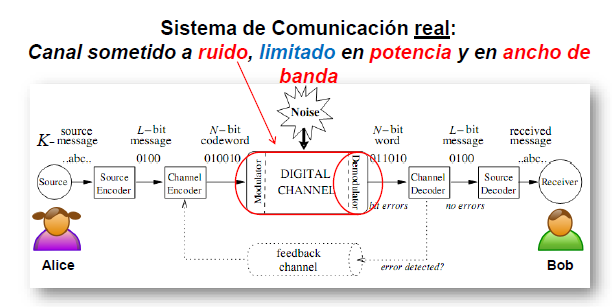
\includegraphics[width=0.65\textwidth
]{images/sistema-comunicacion-real.png}
	\caption[Esquema general de un sistema de comunicación]{Esquema general de un sistema de comunicación}
	\label{fig:sistema-comunicacion-correccion}
\end{figure}

Una forma de tratar de resolver esto es agregar al modelo nuevas capas de actores que trabajan para reducir los efectos nocivos del ruido. Por ejemplo, podemos agregar al modelo observadores externos que sean capaces de ver lo que se transmite de un lado y se recibe del otro, deducir información a partir de las diferencias, y tener chance de enviarle
correcciones al Elemento Corrector. También es posible tener dos niveles de observadores:
uno que se maneja a nivel mensaje y otro que se maneja a nivel característica del canal
propio.

\subsubsection{Tipos de errores de los canales físicos}
\begin{itemize}
  \item \textbf{Atenuación:}  En medios análogicos, la señales se degradan con la distancia recorrida lo que puede llevar a provocar errores en algunos bits recibidos. Por lo que la intensidad de la señal recibida deber ser suficiente para ser detectada y, además, debe ser suficientemente mayor al ruido del canal para que se reciba sin error. En general, las frecuencias más afectadas son las más altas por lo que se puede ecualizar estas frecuencias, es decir, amplificarlas.
  \item \textbf{Distorsión de retardo:} En medios guiados, la velocidad de propagación en el medio varía con la frecuencia por lo que los componentes del mensaje llegan en distintos instantes de tiempo, originando desplazamiento de fases entre las distintas frecuencias. Esto se puede deber a varios motivos.
\item \textbf{Ruido:} Los canales físicos poseen ruido natural. Es decir, transmiten señales adicionales debido a agentes externos:
\begin{itemize}
  \item \textbf{Ruido Término ó Ruido Blanco:} Se produce debido a la agitación térmica de electrones y aumenta linealmente con la temperatura absoluta del canal. En general, está distribuido de manera uniforme a lo largo de todo el canal y para un ancho de banda \(B\), la potencia del ruido blanco \(N_b = kTB\). 
  \item\textbf{Ruido por intermodulación:} Son señales que son la suma o la diferencia de sus frecuencias originales producidas por una falta de linealidad en el canal. \(N_I = m f_1 \pm n f_2\)
  \item\textbf{Ruido por Diafonía:} Se produce cuando una señal de una línea interfiere en otra.
  \item\textbf{Ruido impulsivo:} Son impulsos irregulares o picos que se pueden producir por interferencias externas (como pueden ser interferencia electromagnéticas, tormentas, etc). Este tipo de ruido es de corta duración, tienen gran amplitud y es disruptivo.
\end{itemize}
\end{itemize}

\subsubsection{Capacidad de un canal}
Las perturbaciones mencionadas afectan la velocidad de transmición del canal por lo que debemos asegurarnos de no enviar más bits que la capacidad límite del mismo para no perder información durante la transmición. Para esto vamos a definir los siguientes conceptos:

\begin{itemize}
  \item \(C\) es la capacidad del canal o tasa de datos, es decir a la cantidad de bits por segundo que podemos transmitir a través del mismo.
  \item \(B\) es el ancho de banda por el cual vamos a transmitir nuestros datos, va estar medido en ciclos por segundo (Hertz) y va estar limitado por el transmiso y el medio.
  \item \(N\) es el nivel medio o potencia del ruido del canal
  \item \(BER\) es la tasa de errores de bits por segundo (Bit Error Rate).
  \item \(S\) es la potencia o amplitud de la señal.
  \item \(SNR = S / N\) es la cantidad de ruido térmico presente se mide por la relación entre la potencia de la señal y la potencia del ruido, llamada relación señal a ruido. Por lo general, la relación misma no se expresa; en su lugar, se da la cantidad \(10 \log_{10} S/N\).
  Estas unidades se conocen como decibeles (dB).
\end{itemize}

En un canal sin ruido, \(C = 2B\log_2 M\) donde \(M\) es la cantidad de niveles que usamos para representar los símbolos.

En un canal con ruido, Shannon propuso
\[C_{max} = B\log_2(1 + SNR)\]

En principio, si se aumentan el ancho de banda \(B\) y la potencia de señal \(S\), aumenta la velocidad binaria. Sin embargo, un aumento de \(B\) aumenta el ruido y un aumento de \(S\) aumenta las no linealidades y el ruido de intermodulación.

\begin{figure}[H]
	\centering
	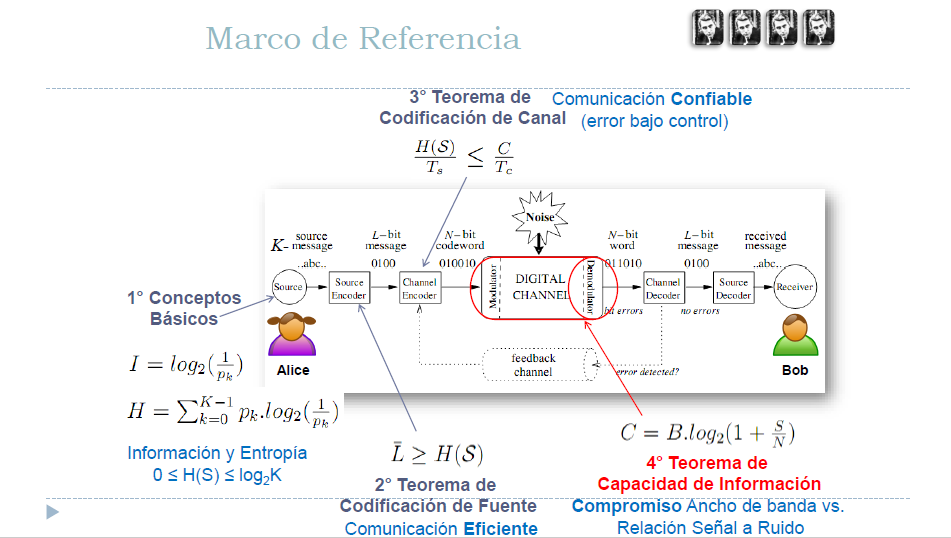
\includegraphics[width=\textwidth
]{images/marco-referencia.png}
	\caption[Esquema de un sistema de comunicación y sus conceptos asociados]{Esquema de un sistema de comunicación y sus conceptos asociados}
	\label{fig:marco-referencai}
\end{figure}


\paragraph{Límite de eficencia:} La eficiencia de ancho de banda es la máxima cantidad de bits por segundo que podemos inyectar por cada Hz sin perder información. Mientra más eficiente sea el canal, se pueden transmitir más bits por segundo. 

\paragraph{Límie de confiabilidad:} \red{Es la cantidad máxima de bits por segundos que podemos utilizar para transportar una señal de manera confiable a través de un canal ruidoso}

\subsubsection{Delay}
Por último, debemos analizar el tiempo que tarda en llegar un paquete completo desde una punta a otra de la conexión. Este tiempo se ve afectado por varias cosas:
  \begin{itemize}
    \item \textbf{Retardo de procesamiento:} Tiempo requerido en analizar el encabezado y decidir a dónde enviar el paquete. En un enrutador, dependerá del número de entradas en la tabla de rutas, la implementación (estructuras de datos), el hardware, etc. Puede incluir la verificación de errores.
    \item \textbf{Retardo de encolamiento:} Tiempo en que el paquete espera en un buffer hasta ser transmitido. El número de paquetes esperando en cola dependerá de la intensidad y la naturaleza del tráfico. Los algoritmos de colas en los enrutadores intentan adaptar estos retardos a ciertas preferencias, o imponer un uso equitativo.
    \item \textbf{Retardo de transmición:} El tiempo requerido para “empujar” todos los bits de un paquete a través del medio de transmisión. Si \(R\) es la capidad del canal, \(L\) la longitud del paquete y \(D_T\) el delay o retardo de transmición:
    \[D_T = \frac{L}{R}\]
    \item \textbf{Retardo de propagación:} Una vez que el bit es 'empujado' en el medio, el tiempo transcurrido en su propagación hasta
    el final del trayecto físico. La velocidad de propagación del enlace depende más que nada de la distancia medio físico. Si \(d\) es la distancia a recorrer y \(s\) la velocidad de propagación:
    \[D_p = \frac{d}{s}\]
  \end{itemize}

 \subsection{Medios de transmición}
 \subsubsection{Medios guiados}
 \subsubsection*{Par trenzado de cobre} Uno de los medios de transmisión más viejos, y todavía el más común. Éste consiste en dos alambres de cobre aislados, por lo regular de 1 mm de grueso. Los alambres se trenzan en forma helicoidal, igual que una molécula de DNA. Esto se hace porque dos alambres paralelos constituyen una antena simple. Cuando se trenzan los alambres, las ondas de diferentes vueltas se cancelan, por lo que la radiación del cable es menos efectiva.

La aplicación más común del cable de par trenzado es en el sistema telefónico. Casi todos los teléfonos están conectados a la compañía telefónica mediante un cable de par trenzado. La distancia que se puede recorrer con estos cables es de varios kilómetros sin necesidad de amplificar las señales, pero para distancias mayores se requieren repetidores.
    
Se pueden utilizar para transmisión tanto analógica como digital. 

El ancho de banda depende del grosor del cable y de la distancia que recorre; en muchos casos pueden obtenerse transmisiones de varios megabits/seg, en distancias de pocos kilómetros.

\subsubsection*{Coaxial}
Consiste en un alambre de cobre rígido como núcleo, rodeado por un material aislante. El aislante está forrado con un conductor cilíndrico, que con frecuencia es una malla de tejido fuertemente trenzado. El conductor externo se cubre con una envoltura protectora de plástico.

La construcción y el blindaje del cable coaxial le confieren una buena combinación de ancho de banda alto y excelente inmunidad al ruido. El ancho de banda posible depende de la calidad y longitud del cable, y de la relación señal a ruido de la señal de datos. Los cables modernos tienen un ancho de banda de cerca de 1 GHz. Los cables coaxiales solían ser ampliamente usados en el sistema telefónico para las líneas de larga distancia, pero en la actualidad han sido reemplazados
por la fibra óptica en rutas de distancias considerables. Sin embargo, el cable coaxial aún se utiliza ampliamente en la televisión por cable y en las redes de área metropolitana.

\subsubsection*{Fibra óptica:}
Un sistema de transmisión óptico tiene tres componentes: la fuente de luz, el medio de trans-
misión y el detector. Convencionalmente, un pulso de luz indica un bit 1 y la ausencia de luz in-
dica un bit 0. El medio de transmisión es una fibra de vidrio ultradelgada. El detector genera un
pulso eléctrico cuando la luz incide en él. Al agregar una fuente de luz en un extremo de una fi-
bra óptica y un detector en el otro, se tiene un sistema de transmisión de datos unidireccional que
acepta una señal eléctrica, la convierte y transmite mediante pulsos de luz y, luego, reconvierte la
salida a una señal eléctrica en el extremo receptor.

Cuando un rayo de luz pasa por un medio a otro —por ejemplo, de sílice fundida al aire—, el rayo se refracta (se dobla) en la frontera de la sílice y el aire. Un rayo de luz que incide en la frontera con un ángulo \(\alpha_1\) y que emerge con un ángulo \(\beta_1\). El grado de refracción depende de las propiedades de los dos medios (en particular sus índices de refracción). Para ángulos con incidencias mayores de ciertos valores críticos, la luz se refracta nuevamente a la sílice; ninguna parte de él escapa al aire. Por lo tanto, un rayo de luz que incide en un ángulo mayor o igual que el crítico queda atrapado den-
tro de la fibra.

Puesto que cualquier rayo de luz que incida en la frontera con un ángulo mayor que el crítico se reflejará internamente, muchos rayos estarán rebotando con ángulos diferentes. Se dice que cada rayo tiene un
modo diferente, por lo que una fibra que tiene esta propiedad se denomina \textbf{fibra multimodo}. Por otro lado, si el diámetro de la fibra se reduce a unas cuantas longitudes de onda de luz, la fibra actúa como una guía de ondas y la luz se puede propagar sólo en línea recta, sin rebotar, lo cual da como resultado una \textbf{fibra monomodo}. 

Las fibras monomodo son más caras, pero se pueden utilizar en distancias más grandes. Las fibras monomodo disponibles en la actualidad pueden transmitir datos a 50 Gbps a una distancia de 100 km sin amplificación.

\subsubsection{Medios inalámbricos}
\subsubsection*{El espectro electromagnético}
\begin{figure}[H]
	\centering
	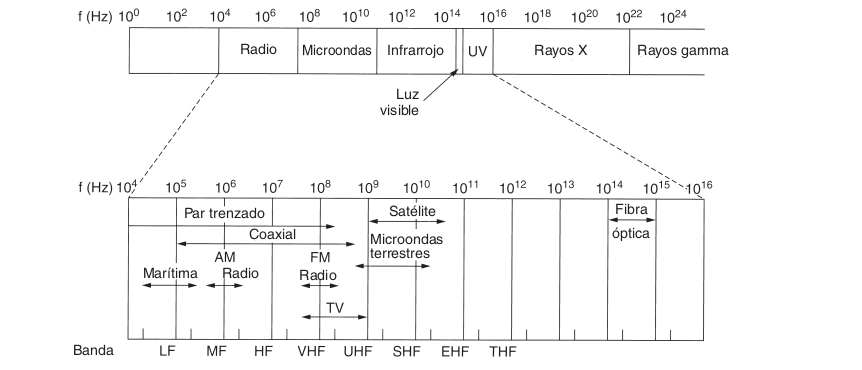
\includegraphics[width=\textwidth
]{images/espectro-magnetico.png}
	\caption[Espector magnetico]{Espector magnetico}
	\label{fig:espectro-magnetico}
\end{figure}

Las porciones de radio, microondas, infrarrojo y luz visible del espectro pueden servir para transmitir información modulando la amplitud, frecuencia o fase de las ondas. La luz ultravioleta, los rayos X y los rayos gamma serían todavía mejores, debido a sus frecuencias más altas, pero son difíciles de producir y modular, no se propagan bien entre edificios y son peligrosos para los seres vivos. 

La cantidad de información que puede transportar una onda electromagnética se relaciona con su ancho de banda. Con la tecnología actual, es posible codificar unos cuantos bits por hertz a frecuencias bajas, pero a frecuencias altas el número puede llegar hasta 8, de modo que un cable coaxial con un ancho de banda de 750 MHz puede transportar varios gigabits/seg.

A las bandas más altas se les nombró como bandas VHF (frecuencia muy alta), UHF (frecuencia ultraalta), EHF (frecuencia extremadamente alta) y THF (frecuencia tremendamente alta).

\subsubsection*{Radio}
Las ondas de radio son fáciles de generar, pueden viajar distancias largas y penetrar edificios sin problemas, y por ello su uso está muy generalizado en la comunicación, tanto en interiores como en exteriores. Las ondas de radio también son  omnidireccionales, lo que significa que viajan en todas direcciones a partir de la fuente, por lo que no es necesario que el transmisor y el receptor se encuentren alineados físicamente.

Las propiedades de las ondas de radio dependen de la frecuencia. A bajas frecuencias, esas ondas cruzan bien casi cualquier obstáculo, pero la potencia se reduce de manera drástica a medida que se aleja de la fuente.

En las bandas VLF, LF y MF las ondas de radio siguen la curvatura de la Tierra. Estas ondas se pueden detectar quizá a 1000 km en las frecuencias más bajas, y a menos en frecuencias más altas.

n las bandas HF y VHF, las ondas a nivel del suelo tienden a ser absorbidas por la tierra. Sin
embargo, las ondas que alcanzan la ionosfera, una capa de partículas cargadas que rodea a la Tie-
rra a una altura de 100 a 500 km, se refractan y se envían de regreso a nuestro planeta. En ciertas condiciones atmosféricas, las señales pueden rebotar va-
rias veces. Los operadores de radio aficionados usan estas bandas para conversar a larga distancia.
El ejército se comunica también en las bandas HF y VHF.

\subsubsection*{Láser}
La señalización óptica coherente con láseres es inherentemente unidireccional, de modo que cada edificio necesita su propio láser y su propio fotodetector. Este esquema ofrece un ancho de banda muy alto y un costo muy bajo. También es relativamente fácil de instalar.

Una desventaja es que los rayos láser no pueden penetrar la lluvia ni la niebla densa, pero nor-
malmente funcionan bien en días soleados. Sin embargo, el calor del sol causa corrientes de convección que se elevabn desde el techo de los edificio. Este aire turbulento desviaba el rayo y lo hacía danzar alrededor del detector.

\subsubsection*{Satélites}
Los satélites de comunicaciones tienen algunas propiedades interesantes que los hacen atrac-
tivos para muchas aplicaciones. En su forma más simple, un satélite de comunicaciones se puede
considerar como un enorme repetidor de microondas en el cielo. Contiene numerosos transpon-
dedores, cada uno de los cuales se encarga de una parte del espectro, amplifica la señal entrante
y a continuación la retransmite en otra frecuencia para evitar interferencia con la señal entrante.
Los haces pueden ser amplios y cubrir una fracción sustancial de la superficie de la Tierra, o es-
trechos, y abarcar sólo algunos cientos de kilómetros de diámetro. Este modo de operación se
conoce como de tubo doblado.

\subsection{Red télefonica}
La \textbf{Red Telefónica Pública Conmuta-
da} (PSTN), fue diseñadas hace muchos años, con el propósito de transmitir la voz humana en una forma más o menos reconocible.

\begin{figure}[H]
	\centering
	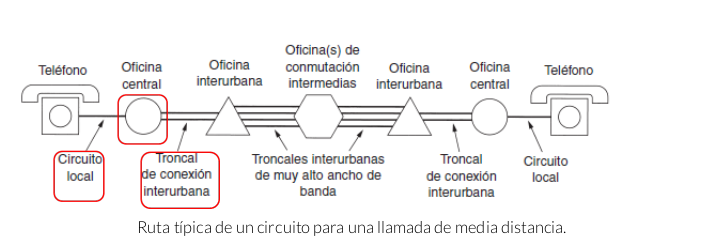
\includegraphics[width=0.9\textwidth
]{images/redes-telefonicas.png}
	\caption[Sistema  telefónico]{Sistema  telefónico}
	\label{fig:sistema-telefonico}
\end{figure}

El sistema telefónico consiste en tres componentes principales:
\begin{enumerate}
  \item Circuitos locales: Cables de par trenzado que van hacia las casas y las empresas. Dan acceso a todo mundo al sistema completo, debido a lo cual son cruciales. Por desgracia, también son la parte más débil del sistema. Cada oficina central tiene varias líneas salientes a uno o más centros de conmutación cercanos, llamados \textbf{oficinas interurbanas}.
  \item Troncales (fibra óptica digital que conecta a las oficinas de conmutación).
  \item Oficinas de conmutación (donde las llamadas pasan de una troncal a otra).
\end{enumerate}

Para las troncales de largo alcance, la principal consideración es cómo reunir múltiples llamadas y
enviarlas juntas por la misma fibra. Este tema se llama \textbf{multiplexión}.

\subsubsection{Tipos de multiplexión}
Las compañías telefónicas han desarrollado esquemas complejos para multiplexar muchas conversaciones en una sola troncal física. Estos esquemas de multiplexión se pueden dividir en dos categorías principales: FDM (Multiplexión por División de Frecuencia) y TDM (Multiplexión por División de Tiempo). En FDM el espectro de frecuencia se divide en bandas de frecuencia, y cada usuario posee exclusivamente alguna banda. En TDM los usuarios esperan su turno (en round-robin), y cada uno obtiene en forma periódica toda la banda durante un breve lapso de tiempo.

\paragraph{Multiplexión por División de Frecuencia:} Los filtros limitan el ancho de banda utilizable a cerca de 3000 Hz por canal de calidad de voz. Cuando se multiplexan muchos canales juntos, se asignan 4000 Hz a cada canal para mantenerlos bien separados. Primero se eleva la frecuencia de los canales de voz, cada uno en una cantidad diferente, después de lo cual se pueden combinar, porque en ese momento no hay dos canales que ocupen la misma porción del espectro. Hay cierta superposición entre canales adyacentes porque los filtros no tienen bordes bien definidos. Esta superposición significa que un pico fuerte en el borde de un canal se detectará en el adyacente como ruido no térmico. Para los canales de fibra óptica se utiliza una variante de la multiplexión por división de fre-
cuencia llamada \textbf{Multiplexión por División de Longitud de Onda} (WDM).

\paragraph{Multiplexión por División de Tiempo:} Aunque FDM aún se utiliza sobre cables de cobre o canales de microondas, requiere circuitos analógicos y no es fácil hacerla con una computadora. En contraste, TDM puede manejarse por completo mediante dispositivos digitales y a ello se debe su popularidad en los últimos años. Desgraciadamente, sólo se puede utilizar para datos digitales. Puesto que los circuitos locales producen señales analógicas, se necesita una conversión de analógico a digital en la oficina central, en donde todos los circuitos locales individuales se juntan para combinarse en troncales.

\subsubsection{Conversión analógico digital}
\begin{figure}[H]
	\centering
	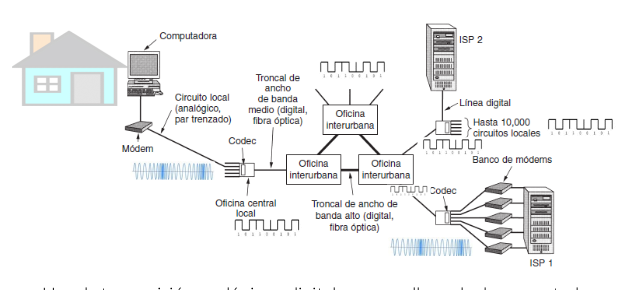
\includegraphics[width=0.9\textwidth
]{images/conversion-analogico-digital.png}
	\caption[Conversión analogico digital]{Conversión analogico digital}
	\label{fig:conversion-analogico-digital}
\end{figure}
\subsection{Modulación}
La transmición analógica se basa en una señal continua de frecuencia constante  denomidada \textbf{portadora}. La frecuencia de la portadora se elige de tal forma que sea compatible con las características del medio que se vaya a utilizar. Los datos se pueden transmitir modulando la señal portadora para asegurarnos de que llegue al próximo extremo sin perder información. Todas las técnicas de modulación implican la modificación de uno o más de los tres parámetros fundamentales de la frecuencia portadora: amplitud, frecuencia y fase.

La señal de entrada \(m(t)\) se denomina señal \textbf{moduladora} a la señal resultante de la modulación de la señal portadora.

Hay distintos tipos de modulaciones:

\begin{itemize}
  \item \textbf{Desplazamiento de amplitud (ASK):} Los dos valores binarios se represnetan mediante dos amplitudes diferences de la portadora. Es usual que una de las amplitudes sea cero.
  \[
    S(t) = \begin{cases}
      A\cos(2\pi f_c t) & \text{1 binario} \\
      0 & \text{0 binario}
    \end{cases}
  \]

  ASK es sensible a cmabios repentinos de la ganancia, además es una técnica de modulación bastante ineficaz. Se usa para la transmición de datos digitales en fibras ópticas
  \item  \textbf{Desplazamiento de frecuencia (FSK):} Los dos valores binarios se representan mediante dos frecuencias diferentes próximas a la frecuencia portadora. La señal resultante es
  \[
    S(t) = \begin{cases}
      A\cos(2\pi f_1 t) & \text{1 binario} \\
      A\cos(2\pi f_2 t) & \text{0 binario}
    \end{cases}
  \]
  
  donde \(f_1\) y \(f_2\) corresponden a desplazamientos de la frecuencia portadora \(f_c\), de igual magnitud pero en sentidos opuestos.

  FSK es menos sensible a errores que ASK.
  \item  \textbf{Desplazamiento de fase (PSK):} La fase de la señal portadora se despaza para representar con ello a los datos digitales: En este sistema, un cero binario se representa mediante la transmición de una señal con la misma fase que la fase de la señal anteriormente enviada. Mientras que un uno se representa mediante la transmición de una señal cuya fase esté en opociión de fase respecto de la señal precente. Esta técnica se conoce como PSK diferencial, ya que el desplazamiento en fase es relativo a la fase correspondiente al último símbolo transmitido.
  
  \[
    S(t) = \begin{cases}
      A\cos(2\pi f_c t + \pi) & \text{1 binario} \\
      A\cos(2\pi f_c t) & \text{0 binario}
    \end{cases}
  \]
\end{itemize}

\paragraph{Velocidad de modulación:} El número de cambios de señal por unidad de tiempo. Se expresa en \textbf{baudios} (símbolos por segundo).

\paragraph{Velocidad de transmición:} Equivale a la velocidad de modulación multiplicado por el número de bits \(N\) represenntados por cada símbolo. Se expresa en bits por segundo: \(V_t = V_m\cdot m\)

Se puede conseguir una utilización más eficaz del ancho de banda si cada elemento de señalización representa más de un bit.  En el métood PSKQ  considera desplazamientos de fase correspondientes a \(\pi/2\) (\(90°\)) por lo que cada señal representa dos bits en lugar de uno:
\[
  S(t) = \begin{cases}
    A\cos(2\pi f_c t + \frac{\pi}{4}) & \text{11} \\
    A\cos(2\pi f_c t + \frac{3\pi}{4}) & \text{10} \\
    A\cos(2\pi f_c t + \frac{5\pi}{4}) & \text{00} \\
    A\cos(2\pi f_c t + \frac{7\pi}{4}) & \text{01} \\
  \end{cases}
\]

\subsubsection{Codificación}
Una vez modulada, la señal analógica viaja hasta un \textbf{codec}  en la oficina central  que se encarga de digitalizarla. El codec toma 8000 muestras por segundo porque el teorema de Nyquist dice que esto es suficiente para capturar toda la información del ancho de banda de 4 kHz del canal telefónico. A una velocidad de muestreo menor, la información se perdería; a una mayor, no se ganaría información extra. Esta técnica se llama \textbf{Modulación por Codificación de Impulsos} (PCM).   

A veces, se usa un técnica conocida como \textbf{Modulación Delta}, en el que la entrada analógica se aproima mediante una función escalera que en cada intervalo de muestreo (\(T_S\)) sube o bajaa un nivel de cuantización \(\delta\). La característica principal de la función escalera es qeu su comportamiento es binario: En cada instante de muestreo, la función sube o baja una cantidad constante. Por tanto, la salida del modulador delta se puede representar mediante un único bit para cada muestra. Resumiendo: se obiente una cadena de bits que aproxima a la derivada de la señal analógica de entrada en cualquier lugar de la amplitud.

\subsubsection*{No retorno a cero (NRZ)}
La forma más frecuente y fácil de transmitir señales digitales es mediante la utilización de un nivel diferente de tensión para cada uno de los dos dígitos binatios. Los códigos que siguen esta estrategia comparten la propiedad de que el nivel de tensión se mantiene constante durante la duración del bit. Es habitual usar un nivel negativo para representar un valor binario y un tensión positiva para representar el otro.

Una variante de este código de nomina \textbf{No retono a Cero con Inversion de unos} (NZRI) en la que un 1 se codifica mediante la transición al principio del intervalo de señalización, mientras que un 0 se rpresenta por la ausencia de transición. Esta codificación es un ejemplo de codificación diferencial, en lugar de determinar el valor absoluto, la señal se codifica comparando la polaridad de los elementos de señal adyacentes.

\subsubsection*{Codificación Manchester (Bifase)}
El valor de un bit se códifica en una transición a la mitad del intervalo de duración del bit. Esta transición en la mitad del bit sirve como un procedimiento de sincronización a la vez que sirve para transmitir los datos: Una transción de bajo a alto representa un 1 y una transición de alto a bajo representa un cero.

En Mancheste diferencial, la transición a mitad del intervalo se utiliza tan solo para proporcionar sincronización. La codificación de un cero se representa por la presencia de una trancisión al principio del intervalo. 

Toda técnica bifase fuerzan al menos una transición por cada bit pudiendo tener hasta dos en ese mismo período. Por tanto, la velocidad de modulación máxia es el doble que en los NRZ y el ancho de banda necesario es mayor.

\subsection{Redes de conmutación}
En la actualidad se utilizan dos técnicas de conmutación diferentes: conmutación de circuitos y conmutación de paquetes. A continuación presentaremos una breve introducción a cada una de ellas.

\subsubsection*{Conmutación de circuitos}
Cuando se realiza una llamada telefónica, el equipo de conmutación del sistema telefónico busca una trayectoria física que vaya desde su teléfono al del receptor. Esta técnica se llama \textbf{conmutación de circuitos}.

Una propiedad importante de la conmutación de circuitos es la necesidad de establecer una trayectoria de un extremo a otro antes de que se pueda enviar cualquier dato. El tiempo que transcurre entre que se termina de marcar y que el timbre comienza a sonar puede ser fácilmente de 10 seg, y más en las llamadas de larga distancia o internacionales. Durante este intervalo de tiempo, el sistema telefónico busca una trayectoria de cobre. La señal de petición de llamada se debe propagar hasta el destino y se debe confirmar su recepción. En muchas aplicaciones de computadora, los tiempos de establecimiento largos son indeseables.

Por otro lado, al existir una trayectoria de cobre entre las partes en comunicación, una vez que se termina de establecer, el único retardo de los datos es el tiempo de propagación de la señal electromagnética y no
hay peligro de congestión; es decir, una vez que la llamada entra, no hay posibilidad de obtener una señal de ocupado, aunque podría obtener una antes de establecer la conexión debido a la falta de capacidad de conmutación o de troncal.

\subsubsection*{Conmutación de paquetes}
La alternativa a la conmutación de circuitos es la \textbf{conmutación de paquetes}. Con esta tecnología, los paquetes individuales se envían conforme se necesite, y no se les asigna por adelantado ninguna trayectoria dedicada.

En este caso, al no ser necesaria una conexión previa, el primer paquete se puede enviar apenas esté listo. 

Con la conmutación de paquetes no
hay trayectoria, por lo que diferentes paquetes pueden seguir trayectorias distintas, dependiendo
de las condiciones de la red en el momento en el que se enviaron. Pueden llegar en desorden.

La conmutación de paquetes es más tolerante a las fallas que la conmutación de circuitos. De  hecho, ésa es la razón por la cual se inventó. Si falla la conmutación, todos los circuitos que la están utilizando se cancelan y no se puede enviar nada más a través de ellos. Con la conmutación de pa-
quetes, los paquetes pueden enrutarse evitando a los conmutadores averiados.

La conmutación de paquetes utiliza transmisión de almacenamiento y reenvío. Un paquete se
almacena en la memoria del enrutador y luego se reenvía al siguiente enrutador. Con la conmuta-
ción de paquetes los bits simplemente fluyen de manera continua a través del cable. La técnica de
almacenamiento y reenvío agrega retardo.

\newpage
\section{Nivel de enlace}
La capa de enlace de datos tiene que desempeñar varias funciones específicas, entre las que
se incluyen:
\begin{itemize}
  \item Proporcionar una interfaz de servicio bien definida con la capa de red.
  \item Manejar los errores de transmición.
  \item Regular el flujo de datos para que receptores lentos no sean saturados por emisores rápidos.
\end{itemize}
Para cumplir con estas metas, la capa de enlace de datos toma de la capa de red los paquetes y los encapsula en \textbf{tramas} para transmitirlos. Cada trama contiene un \textbf{encabezado}, un campo de carga útil (\textbf{payload}) para almacenar el paquete y un \textbf{terminador} o final. El manejo de las tramas es la tarea primordial de la capa de enlace de datos.

\subsection{Servicios proporcionados}
La capa de enlace de datos puede diseñarse para ofrecer varios servicios. Los servicios reales
ofrecidos pueden variar de sistema a sistema. Tres posibilidades razonables que normalmente se
proporcionan son:
\begin{enumerate}
  \item \textbf{Servicio no orientado a la conexión sin confirmación de recepción:} Consiste en hacer que la máquina de origen envíe tramas independientes a la máquina de destino sin pedir que ésta confirme la recepción. No se establece conexión de antemano ni se libera después. Si se pierde una trama debido a ruido en la línea, en la capa de enlace de datos no se realiza ningún intento por detectar la pérdida ni por recuperarse de ella.
  \item \textbf{Servicio no orientado a la conexión con confirmación de recepción:} Cuando se ofrece este servicio tampoco se utilizan conexiones lógicas, pero se confirma de manera individual la recepción de cada trama enviada. De esta manera, el emisor sabe si la trama ha llegado bien o no. Si no ha llegado en un tiempo especificado, puede enviarse nuevamente.
  \item \textbf{Servicio orientado a la conexión con confirmación de recepción:} Con este servicio, las máquinas de origen y de destino establecen una conexión antes de transferir datos. Cada trama enviada a través de la conexión está numerada, y la capa de enlace de datos garantiza que cada trama enviada llegará a su destino. Es más, garantiza que cada trama será recibida exactamente una vez y que todas las tramas se recibirán en el orden adecuado.
\end{enumerate}

\subsection{Separación de frames:}
Puesto que es demasiado riesgoso depender de la temporización para marcar el inicio y el final de cada trama, se han diseñado otros métodos:

\begin{enumerate}
  \item \textbf{Largo fijo:} Todos los paquetes tienen la misma longitud.
  \item \textbf{Conteo de caracteres}: Se vale de un campo en el encabezado para especificar el número de caracteres en la trama. Cuando la capa de enlace de datos del destino ve la cuenta de caracteres, sabe cuántos caracteres siguen y, por lo tanto, dónde está el fin de la trama. El problema con este algoritmo es que la cuenta puede alterarse por un error de transmisión. Si esto pasa, el destino perderá la sincronía y será incapaz de localizar el inicio de la siguiente trama. Incluso si el destino sabe que la trama está mal porque la suma de verificación es incorrecta, no tiene
  forma de saber dónde comienza la siguiente trama. Regresar una trama a la fuente solicitando una retransmisión tampoco ayuda, ya que el destino no sabe cuántos caracteres tiene que saltar para llegar al inicio de la retransmisión.
  \item \textbf{Flags con bit-stuffing}: El segundo método de entramado evita el problema de tener que sincronizar nuevamente después de un error, haciendo que cada trama inicie y termine con bytes especiales llamado \textbf{flags}. De esta manera, si el receptor pierde la sincronía simplemente puede buscar la bandera para encontrar el final e inicio de la trama actual. Dos banderas consecutivas señalan el final de una trama y el inicio de la siguiente. 
  
  Cuando se utiliza este método para transmitir datos binarios, como programas objeto o números de punto flotante, surge un problema serio. Se puede dar el caso con mucha facilidad de que el patrón de bits de la bandera aparezca en los datos (payload), lo que interferiría en el entramado. Una forma de resolver este problema es hacer que la capa de enlace de datos del emisor inserte un byte de \textbf{escape especial} (ESC) justo antes de cada bandera “accidental” en los datos. La capa de enlace de datos del lado receptor quita el byte de escape antes de entregar los datos a la capa de red. Esta técnica se llama \textbf{relleno de caracteres} o bit-stuffing. Por lo tanto, una bandera de entramado se puede distinguir de uno en los datos por la ausencia o presencia de un byte de escape que la antecede.
\end{enumerate}

\subsection{Detección y corrección de errores}

Los diseñadores de redes han desarrollado dos estrategias principales para manejar los errores. Una es incluir suficiente \textbf{información redundante} en cada bloque de datos transmitido para que el receptor pueda deducir lo que debió ser el carácter transmitido. La otra estrategia es incluir sólo suficiente redundancia para permitir que el receptor sepa que ha ocurrido un error (pero no qué error) y entonces solicite una retransmisión. La primera estrategia utiliza \textbf{códigos de corrección de errores}; la segunda usa \textbf{códigos de detección de errores}. 

\subsubsection{Detección de errores}
\paragraph{Bit de paridad:} La forma más sencilla. Consiste en añadir un bit de paridad al final del bloque de datos. El valor de ese bit se determina de tal forma que el código resultante tenga un número impar de unos. El receptor examina el código recibido y, si el número total es impar, supondrá que no ha habido errores. 

La utilización de bits de paridad no es infalibre, ya que los impulsos de ruido son a veces lo suficientemente largos como para destruir más de un bit.

\paragraph{Comprobación de redundancia cíclica (CRC):} Dado un bloque o mensaje de \(k\)-bits, el trasmisor genera una secuencia de \(n\)-bits denominada \textbf{secuencia de comprobación de la trama} de tal manera que la trama resultante con \(n+k\) bits, se divisible por algún número determinado. El receptor entonces divirá la trama recibida por ese número y, si no hay resto en la división, se supone que no ha habido errores.

\subsubsection{Códigos de corrección de errores}
Por lo general, una trama consiste en \(m\) bits de datos (es decir, de mensaje) y \(r\) bits redundantes o de verificación. Sea la longitud total \(n\) (es decir, \(n = m + r\)). A una unidad de \(n\) bits que contiene datos y bits de verificación se le conoce como palabra codificada de \(n\) bits.

Dadas dos palabras codificadas cualesquiera es posible determinar cuántos bits correspondientes difieren aplicando un OR exclusivo a las dos palabras codificadas y contar la cantidad de bits 1 en el resultado. La cantidad de posiciones de bits en la que difieren dos palabras codificadas se llama \textbf{distancia de Hamming}. Si dos palabras codificadas están separadas una distancia de Hamming \(d\), se requerirán \(d\) errores de un bit para convertir una en la otra.  

Para detectar \(e\) errores se necesita un código con distancia \(e + 1\), pues con tal código no hay manera de que \(e\) errores de un bit puedan cambiar una palabra codificada válida a otra. Cuando el receptor ve una palabra codificada no válida, sabe que ha ocurrido un error de transmisión. De manera similar, para corregir \(e\) errores se necesita un código de distancia \(2e + 1\), pues así las palabras codificadas legales están tan separadas que, aun con \(e\) cambios, la palabra codificada original sigue estando más cercana que cualquier otra palabra codificada, por lo que puede determinarse de manera única. 

\subsection{Protocolos de Transmición confiable}
\subsubsection{Stop \& Wait}
\begin{figure}[H]
	\centering
	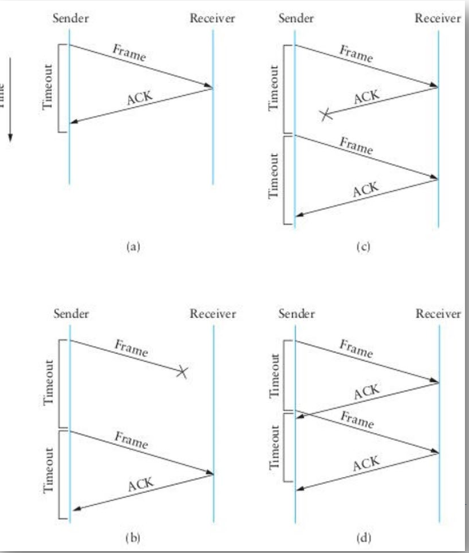
\includegraphics[width=0.65\textwidth
]{images/stop-wait.png}
	\caption[Protocolo Stop And Wait]{Protocolo Stop And Wait}
	\label{fig:stop-wait}
\end{figure}
La máquina de origen emite un único frame y espera la recepción de una confirmación (ACKnowledgment) durante un período determinado de tiempo \(t\). Mientras tanto no podrá enviar ningún otro frame.


Pueden surgir dos problemas durante la comunicación:
  
El receptor detecta algún error, entonces descartará el frame y no manda el ACK. El temporizador expira antes de la recepción del ACK y re-envía el último frame.

Por otro lado, si el frame llega correctamente y el receptor envía una ACK pero el ACK se pierde en el camino, tambien expira el temporizado y el origen vuelve a enviar el mismo frame. 
  
El destino recibe por segunda vez el frame como si fuese un frame distinto.

Para evitar este problema, los frames se etiquentan alternadamente con 0  1, y las confirmaciones positivas serán de la forma ACK0 y ACK1. Un ACK0 confirma la recepción de un frame numerada con 0 e indica que el receptor está esperando para aceptar un frame numerado con 0.

Ahora, cuando el receptor reciba dos frames con la misma numeración, podrá interpretar que está recibiendo un frame duplicado porque su ACK se perdió en el camino. En este caso, el receptor descartará el frame y volverá a mandar el ACK correspondiente.

\paragraph{Eficiencia de un protocolo:} 
Vamos a definir:
\begin{itemize}
  \item \(T_{tx}\) el tiempo de transmición de un frame (lo que tarda en ir desde el origen hasta el destino).
  \item \(RTT(F)\) el tiempo de retorno del ACK, osea el tiempo que tarda en llegar el frame al receptar sumado al tiempo que tarda en llegar el ACK al emisor original. En genaral va a pasar que \(RTT(F) = Delay\times 2\) 
\end{itemize}

El rendimiento de un protocolo \(\eta\) se define como:

\[\eta_{proto} = \frac{T_{tx}(F)}{RTT(F)}\]

\subsection{Ventana deslizante}
Aumentar la eficiencia \(eta\), implica disminuir al minimo la cantidad de tiempo que el origen se bloquea durante la espera de un ACK.

Una estrategia posible para esto es enviar varios frames seguidos, sin esperar ACKs para cada uno.
Aparece el concepto de \textbf{ventana de frames}: en una ventana se envía una cierta cantidad de frames. Esto resulta en una definición diferente para la eficiencia:

\[\eta_{proto} = \frac{T_{tx}(V)}{RTT(F)}\]

donde \(T_{tx}(V)\) es el tiempo de transmición de una ventana.

Sea \(V_{tx}\) la velocidad de transmición, definimos la capacidad de volumen de un canal \(C_{vol} = V_{tx}\times Delay\) como la cantidad de bits que entran en un canal de manera simultáneas sin saturarlo. Con esto, podemos calcular el \textbf{Sliding Window Size (SWS)} de la siguiente manera:

\[SWS = \frac{V_{tx}\times RTT(F)}{|Frames|} \text{ frames}\]

Al comenzar la comunicación, la máquina origen manda \(SWS\) frames al máquina destino. Y espera a recibir el ACK del primer frame enviado. Cuando esto sucede, el origen manda el siguiente frame de la secuencia.

Por cada ACK recibido, el origen va mandando de a uno los frames restantes siempre y cuando el último frame enviado pertezca a una ventana que contenga al frame del último ACK recibido.

\begin{itemize}
  \item \textbf{ACKs Acumulativos:} Si un ACK se pierde, el receptor descarta todos los paquetes hasta que reciba el paquete que está esperando. Esto va a provocar que se produzca un timeout en el emisor del primer paquete perdido y de todos los siguientes, por lo que volverá a enviar todos los frames de nuevo desde el último ACK recibido.
  \item \textbf{ACKs Selectivos:} El receptor recibe y se guarda todos los frames que van llegando. Supongamos que recibe el frame \(i\) con errores. Cuando llega el frame \(i + 1\) responde al receptor con un NAK\(i\). Esto le indica al emisor que si bien recibió el último paquete enviado, hubo un error en el frame anterior y tiene que reenviarlo.
  
  El receptor sigue aceptando frames y respondiendo con ACK\(i-1\) hasta que consigue correctamente el frame perdido. En este momento, responde con un ACK\(j\) donde \(j\) corresponde con el último frame que recibió sin error.
\end{itemize}

Los frames están enumerados de manera cíclica desde 1 hasta \(SWS + RWC\) donde \(RWC\) es el tamaño de la ventana de recepción y se define de la siguiente manera:

\[
  RWC = \begin{cases}
    SWS & \text{si hay ACKs Selectivos} \\
    1 & \text{si hay ACKs Acumulativos}
  \end{cases}
\]

\begin{figure}[H]
	\centering
	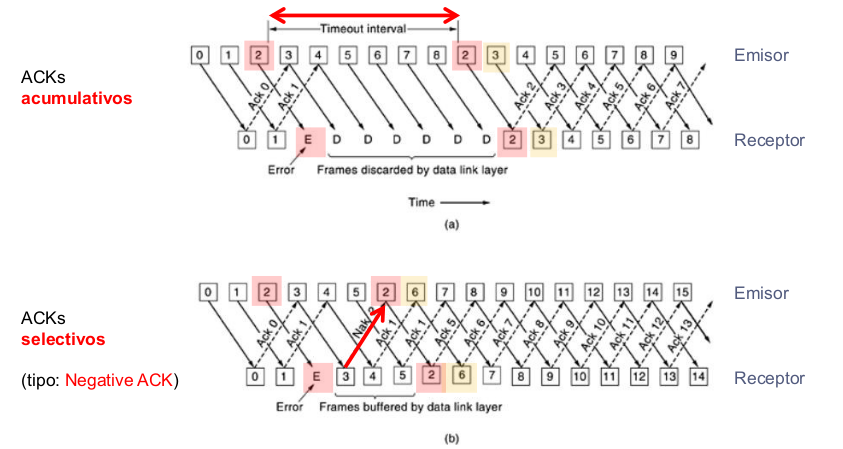
\includegraphics[width=\textwidth
]{images/sliding-window.png}
	\caption[Protocolo Sliding Window]{Protocolo Sliding Window}
	\label{fig:sliding-window}
\end{figure}

\newpage
\section{Medios Compartidos}
La idea es controlar el acceso a los medios compartidos de manera tal que haya la menor cantidad de intervención humana posible en el proceso. Es decir, se busca no tener la figura de un administrador que tenga que solucionar manualmente las cosas.

Tanto TDM, FDM, WDM y CDMA (Code Division Multiple Access) comparten una característica: debe estar decidido a priori qué usuario está usando qué parte del tiempo, frecuencia, etc. en cada momento. Para eso es necesario saber de antemano cuántos usuarios tendrá el sistema. Esto requiere un administrador dedicado a una red con características estáticas, rígidas.

Esto no escala de manera automática, por lo que no cumple la idea mencionada arriba. Esto no significa que estas técnicas no se usen: se utilizan frecuentemente en las redes
troncales (backbones), que no tienen una cantidad constantemente cambiante de nodos como sí puede tener algo como una red LAN, o Wi-Fi. Una alternativa a esto, para redes donde la cantidad de nodos es desconocida y cambiante, es la \textbf{contención estadística}. Esto se refiere a sistemas en los cuales varios usuarios comparten un canal común, de modo tal que puede dar lugar a conflictos conocidos como sistemas de
contención. Estos conflictos son aceptados y/o manejados.

\paragraph{Problemas de acceso:} Si hay varios nodos que usan un medio físico compartido, la simultaneidad de transmisión no es posible (no pueden transmitir todos a la vez). Para esto aparecen los \textbf{MAC Protocols (Medium Access Control)}, protocolos que buscan maximizar, en promedio, el número de éxitos en los intentos de comunicación, y asegurar la igualdad de oportunidades (en promedio) entre todos los nodos competidores.

En estos casos, el control es descentralizado, y surge la necesidad de un esquema de direccionamiento y de controlar el acceso.

Ejemplos: Aloha, Ethernet, Wi-Fi, Token Ring.

\subsection{Ethernet (IIEEE 802.3)}
Las computadoras de un edificio se conectan entre sí por medio de cables. Cada versión de Ethernet tiene un máximo de distancia física entre segmentos. Para permitir conexiones de mayor distancia se pueden utilizar \textbf{repetidores}, que son dispositivos que amplifican y retransmiten señales en ambas direcciones.
El formato utilizado para enviar mensajes en la red es el siguiente:

\begin{figure}[H]
	\centering
	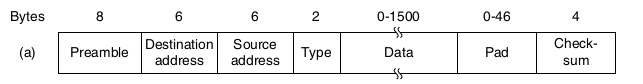
\includegraphics[width=\textwidth
]{images/ethernet-mac-frame.png}
	\caption[Frame del protocolo Ethernet]{Frame del protocolo Ethernet}
	\label{fig:ethernet-mac-frame}
\end{figure}

\begin{itemize}
  \item Los primeros 8 bytes son un preambulo que permiten a los receptors sincronizarse con la señal.
  \item Luego, vienen dos direcciones, cada uno de 6 bytes. 
  
  Cuando el primer bit de la dirección de destino es un 0, significa que el paquete está dirigido a una máquina específica.  Si es un 1, entonces es un dirección grupal: Estas direcciones permiten que varias máquinas escuchen una única dirección y que todas las máquinas pertenecientes al grupo reciban los paquetes dirigidas a esa dirección. Este tipo de envío se llama \textbf{multicasting}. Además, la dirección especial que consiste en todos bits de valor 1 está reservada para hacer \textbf{Broadcasting} (enviar un mensaje a todos los dispositivos de la red).
  \item Los próximos 2 bytes identifican el tipo de protocolo que debe usarse para procesar el contenido del paquete.
  \item Después viene la información per se que puede ocupar hasta 1500 bytes (un valor decidido de manera arbitraria).
  \item Si la data enviada es menor a 46 bytes, se usa padding hasta completar los 46 bytes necesarios para cumplir con los requirimientos de longitud mínima del mensaje. Esta longitud mínima permite que la máquina de origen detecte colisiones durante la transmición, en el caso de haberlas (más adelante explicado).
  \item Los últimos 4 bytes del paquete son un checksum (CRC de 32 bits) que permite detectar si hubo algún error en el frame, si lo hubo, el frame se descarta.
\end{itemize}

\subsubsection{Colisiones}
Una de las razones para tener una longitud mínima de un frame es para evitar que una máquina termine de transmitir el frame antes de que el primer bit haya alcanzado el otro extremo del cable, donde podría colisionar con otro frame.

\begin{figure}[H]
	\centering
	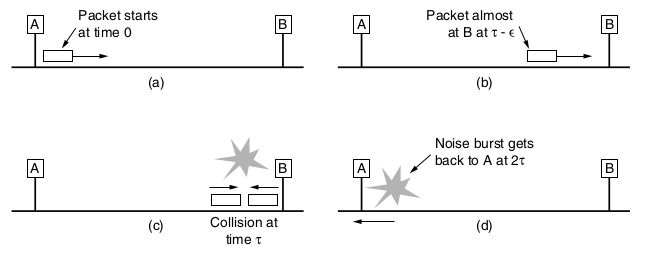
\includegraphics[width=\textwidth
]{images/deteccion-colisiones.png}
	\caption[Detección de Colisiones]{Detección de Colisiones}
	\label{fig:deteccion-colisiones}
\end{figure}

Supongamos que en un timpo 0, el host \(A\) comienza a transmitir el paquete. Sea   \(\tau\) el tiempo de propagación necesario para que el frame llegue al host \(B\). Supongamos que justo antes de que el frame llegue a destino, en el tiempo \(\tau-\epsilon\), \(B\) comienza a transmitir. Cuando \(B\) detecta que está recibiendo más energía que la que está emitiendo, se da cuenta que ocurre una colisión, aborta su propia transmisión y genera una rafaga de sonido ee 48 bits para alertar a las demás estaciones. 

En otras palabras, genera interferencia para asegurarse que el emisor (\(A\)) se de cuenta de que ocurrió la colisión. En el momento \(2\tau\), \(A\) ve el sonido y aborta su propia transmición. Luego espera un intervalo de tiempo random antes de intentar de nuevo.

Si \(A\) trata de enviar un frame muy corto, puede llegar a pasar que termine de trasmitir antes de que  perciba el ruido generado por \(B\) (en el momento \(2\tau\)). Entonces \(A\) concluiria que el frame se envió correctamente. Por esta razón, se utiliza el pading en el frame de Ethernet para completar la longitud mínima de 64 bytes.

Este valor se deduce de las especificacioens de IIEEE 802.3: Para una red de 10Mbps con una longitud de 2500 metros y a lo sumo 4 repetidores, se determinó que el round-trip time es de 50 \(\mu\)segundos, asi que 500 bits es el frame más corto posible para detectar colisiones. Este valor se redondeó a 512 bits (64 bytes).

\subsubsection{CSMA/CD con Exponential BackOff}\label{section::csma}
CSMA/CD (Carrier Sense Multiple Access with Collision Detection), es decir, acceso múltiple con sensado de portadora y detección de colisiones, es un algoritmo de control de acceso a un medio compartido.

Utiliza el sensado de portadora para determinar si hay nodos transmitiendo. Cuando un host tiene datos para enviar, sensa el medio compartido:
\begin{itemize}
  \item Si el medio está libre, el host transmite.
  \item Si el medio está ocupado, no puede enviar porque habría una colisión. Entonces debe esperar a que el medio se libere:
  \begin{itemize}
    \item Si el algoritmo es \textbf{1-persistente}, el host comienza a transmitir apenas se libere el medio.
    \item Si es \textbf{p-persistente}, el host espera a que se libere el medio y transmite con probabilidad \(p\). El uso de un componente azaroso (en la p-persistencia) tiene sentido porque si hay varios
    hosts esperando a que se libere el medio, y todos intentan transmitir ni bien éste se libera, va
    a ocurrir una colisión. Imponer una probabilidad para transmitir reduce las probabilidades de
    colisiones.
  \end{itemize}
\end{itemize}

Este algoritmo es de categoría half-duplex: La lógica de recepción está establecida en el sensado para detectar colisiones. Es decir, no se puede enviar y recibir a la vez (eso sería full-duplex).

Supongamos ahora que ocurre una colisión, entonces el tiempo se divide en slots de tamaño \(2\tau\). Después de la primera colisión, cada estación espera 0 o 1 slots de tiempo al azar. Si dos estaciones colisionan y eligen el mismo número, cada una elige entre 0, 1, 2 ó 3 tiempos al azar y espera el número de slots de tiempos elegidos antes de volver a intentar transmitir.

En general, después de la \(i\)-ésima colisión, cada host debe elegir un número entre 0 y \(2^i-1\) que será la cantidad de slots de tiempo que debe dejar pasar antes de volver a intentar la transmición.

Este algoritmo se llama \textbf{Exponential Backoff Binario}, sirve para adaptar de manera dinámica el número de estaciones que están tratando de emitir simultaneamente. Si el intervalo de elección para todas las elecciones fuese 1023, las chances de colisión son despreciables.


\begin{figure}[H]
	\centering
	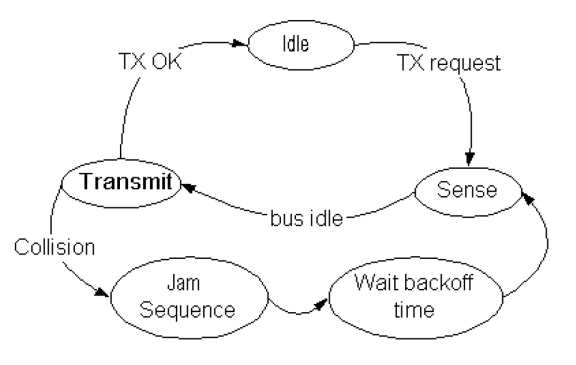
\includegraphics[width=\textwidth
]{images/csma-cd.png}
	\caption[Topologías de Red]{Topologías de Red}
	\label{fig:csma-cd}
\end{figure}

\subsubsection{Logical Link Control}
Es la subcapa de la capa de enlace que se encarga de procesar el paquete recibido en la capa MAC y enviarlo al proceso correspondiente en la capa de Red.

\subsection{Redes inalámbricas: Wi-Fi: IEEE 802.11b/g/n}
En las redes inalámbricas, los frames se mandan a través de ondas en una determinada frecuencia, que depende de la tecnología usada para transmitirlas. En este tipo de red, la intensidad de la señal disminuye con la distancia y tiene fuentes de ruidos más impredecibles que en medios guiados. Esto se traduce en una tasa de errores elevadas.

\subsubsection*{Spread Spectrum}
Esto sumado a que cualquier dispositivo cercarno puede conectarse a ellas, impulsaron el diseño de técnicas para aprovechar al máximo el ancho de banda de tal forma de proteger a la red de intrusos. Est técnica es llamada \textbf{Spread Spectrum}.

Esta técnica modula la señal usando una moduladora semi random compuesta de 1s y -1s conocida por los dispositivos de la red qur aplican a la señal que quieren enviar. Cuando la señal llega el receptor, este realiza el proceso inverso para conseguir la señal original.

Otra forma de realizar esto, es enviar la información transmitida en un rango de frecuencias que es cambiado varías veces durante el proceso de transmición. En este método, la información original se divide en partes más pequeñas usando un patron conocido solamente por el transmisor y el receptor.

\subsubsection{Carrier Sense Multiple Access / Collision Avoidance (CSMA/CA)}

Dado que las redes inalámbricas son un medio de broadcasting, los equipos de la red debe estar atentos a multiples transmiciones realizadas simultaneamente. 
A diferencia de los medios guiados, implementar una comunicación full-duplex sobre radio frecuencias es costoso por lo que se intenta evitar las colisiones en vez de resolverlas.

Para manejar esto, se utiliza el sistema CSMA descripto en la sección \ref{section::csma} pero adaptado a los problemas introducidosra minimizar la probabilidad de colisiones. Si durante este período, el medio se libera, el host puede transmitir una nueva trama. Si no, se vuelve a esperar un nuevo período de contentción. por el nuevo medio que es mucho más lento:

\subsubsection*{Colission Avoidance}
Antes de transmitir, una estación debe determinar el estado del medio. Si el canal no está ocupado, se realiza una espera adicional llamada \textbf{espaciado entre tramas} para asegurarnos de que no colisione.  Si durante esta espera, el medio no permanece libre, entonces se suspende la transmición hasta que se cumpla dicha condición.

Cuando la trama se transmitió, se espera recibir un ACK. Si esto no sucede, se asume que se perdió en una colisión y se retransmitirá la misma. 

Una vez que un host transmite una trama exitosamente, espera un \textbf{período de contención} (cuantificado por un back-off) para minimizar la probabilidad de colisiones. Si durante este período, el medio se libera, el host puede transmitir una nueva trama. Si no, se vuelve a esperar un nuevo período de contención.

Este método recién descripto es llamado \textbf{Distributed Coordination Function (DCF)} y es el método de acceso al medio más básico de 802.11.


\begin{figure}[H]
	\centering
	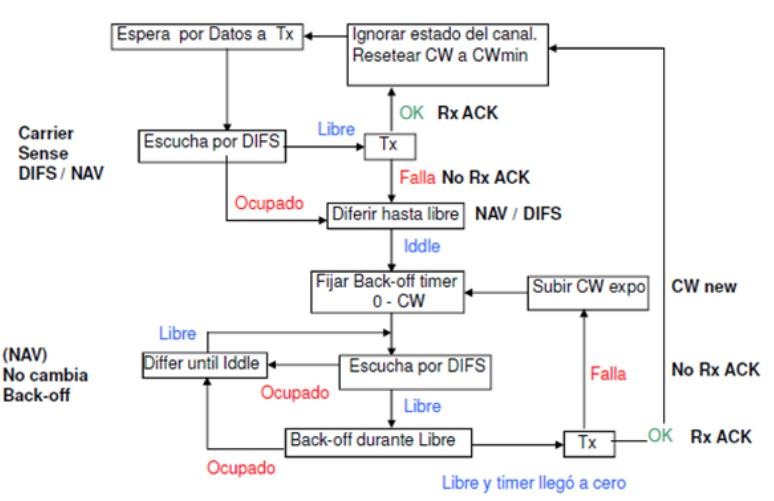
\includegraphics[width=\textwidth
]{images/wifi-estados.jpg}
	\caption[Máquina de estados de un host en una red Wifi]{Máquina de estados de un host en una red Wifi}
	\label{fig:wifi-estados}
\end{figure}

\subsubsection*{Problema de la estación oculta}
Supongamos que la computadora \(A\) comienza a transmitir a \(B\). 

Si \(C\) detecta el medio no escuchará a \(A\) porque está fuera de su alcance, y por lo tanto deducirá erroneamente que puede transmitir. Si lo hace, interferirá en \(B\) eliminando la trama de \(A\).

\begin{figure}[H]
	\centering
	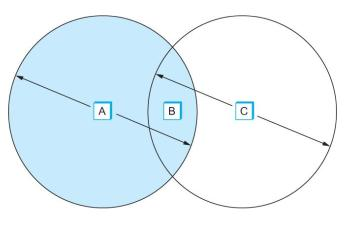
\includegraphics[width=0.5\textwidth
]{images/estacion-oculta.jpg}
	\caption[Problema de la estación oculta]{Problema de la estación oculta}
	\label{fig:estacion-oculta}
\end{figure}

\subsubsection*{Problema de la estación expuesta}
\begin{figure}[H]
	\centering
	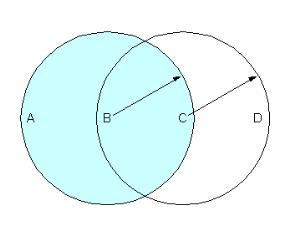
\includegraphics[width=0.5\textwidth
]{images/estacion-descubierta.jpg}
	\caption[Problema de la estación expuesta]{Problema de la estación expuesta}
	\label{fig:estacion-expuesta}
\end{figure}

Supongamos ahora que \(A\) está transmitiendo una tramba a \(B\). Supongamos ahora que \(C\) quiere transmitir a \(D\), cuando detecta al medio, escuhará una transmición y concluirá que no puede realizar su envio. Sin embargo, esa transmición causaría una mala recepción solo en la zona entre \(B\) y \(C\), en la que no está localizado ninguno de los receptores pretendidos.


\newpage
\part{Nivel de Red}
\begin{figure}[H]
	\centering
	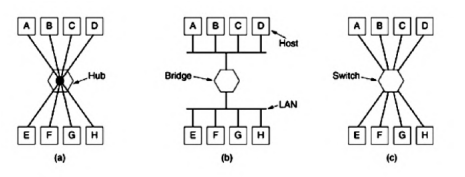
\includegraphics[width=\textwidth
]{images/topologias-red.png}
	\caption[Topologías de Red]{Topologías de Red}
	\label{fig:topologias-red}
\end{figure}
En la figura \ref{fig:topologias-red} se pueden ver tres tipos de LAN:
\begin{enumerate}[a)]
  \item En la primera vemos un conjunto de hosts conectados por un \textbf{hub}, esto es: Todos los hosts están conectado
  s entre sí como si los uniese un único cable. El \textbf{hub}, como los \textbf{repetidores} (amplificadores de señal), funcionan a nivel físico permitiendo agregar equipos a una red.
  \item En el segundo, un puente o \textbf{bridge}, separa en dos grupos los hosts de la red creando dos zonas independientes para la detección de colisiones. En este caso los hosts de un grupo podrán emitir sin tener que preocuparse por interferir con los hosts del otro grupo. Un paquete enviado la dirección de \textbf{broadcast}, alcanza a todos los hosts de la LAN.
  
  Puede interconectar, dos tipos de tecnología distintas (por ejemplo, ethernet y wifi). Por esta razón en la capa MAC, se agrega al header del paquete un campo que permite identificar el tipo de red del que viene. Cuando el bridge capta el paquete y se da cuenta que el host está en una red de distinto tipo, cambia el header para que matcheen y lo reenvía a través de la tecnología correspondiente
  \item Por último tenemos un conjunto de host conectados por un \textbf{switch}: Cada host se conecta con una conexión full-duplex al dispositivo, que se encarga de recibir todos los mensajes de un host y redireccionarlo al host correspondiente. En este tipo de redes se elimina la necesidad detectar colisiones y se pasa a necesitar un algoritmo que permita al switch realizar el dispatch de los mensajes de manera correcta.
  
  Tanto el switch como el bridge funciona a nivel capa de enlace. Se encargan de redireccionar los frames enviados a través de una LAN para que lleguen al dispositivo correspondiente.
\end{enumerate}

Agregamos un último dispositivo: El \textbf{router}, para conectar distintas redes a nivel red. Se encargán de buscar el camino que debe seguir para llegar a destino. Cuando una host envía decide enviar un paquete, lo encapsula en un frame que contiene el tipo de protocolo usado. Cuando el paquete llega el router, este se encarga de tomar el frame que le llego, desencapsular el paquete y guardarlo en un frame adecuado para que pueda ser interpretado por los dispositivos de la nueva ren en la que ingresa el frame.

\section{Switches}
En términos simples, un switch es un mecanismo que nos permite interconectar enlaces para formar una red más grande. Un switch es un dispositivo de múltiples entradas y salidas que transfiere paquetes desde una entrada a una o más salidas. El trabajo principal de un switch es recibir paquetes entrantes en uno de sus enlaces y transmitirlos en otro enlace. Esta función se denomina a veces conmutación (\textbf{switching}) o reenvío (\textbf{forwarding}).

Por lo tanto, un switch agrega la topología de estrella a la topología de enlace punto a punto. Una topología de estrella tiene varias propiedades atractivas:

\begin{itemize}
  \item Aunque un switch tiene un número fijo de entradas y salidas, lo que limita la cantidad de hosts que se pueden conectar a un solo switch, se pueden construir redes grandes interconectando varios switches.
  \item Podemos conectar switches entre sí y a hosts usando enlaces punto a punto, lo que típicamente significa que podemos construir redes de gran alcance geográfico.
  \item Agregar un nuevo host a la red conectándolo a un switch no necesariamente reduce el rendimiento de la red para otros hosts ya conectados.
\end{itemize}

Cada host en una red conmutada (Switched network) tiene su propio enlace al switch, por lo que puede ser completamente
posible que muchos hosts transmitan a la velocidad de enlace completa (ancho de banda),
siempre que el switch esté diseñado con suficiente capacidad agregada.

En general, las redes conmutadas son consideradas más escalables. 

Cuando un router recibe un paquete, busca, en el header del paquete, un identificador que usa para decidir a que puerto. Los detalles de como usa este identificador varían, pero hay dos enfoques comunes. El primero es el enfoque \textbf{datagrama} o \textbf{sin conexión}. El segundo es el enfoque de \textbf{circuito virtual} o \textbf{orientado a conexión}. Un tercer enfoque, el \textbf{enrutamiento de origen} (\textbf{source routing}), es menos común que estos otros dos, pero tiene algunas aplicaciones útiles.

Una cosa que es común a todas las redes es que necesitamos tener una forma de identificar los nodos con los que podremos comunicardos. En general, el identificador que se les asigna se llaman \textbf{direcciones}.

Otra cosa que debemos definir es como el router va a tomar la decisión de a que puerto enviar el paquete. Para esto, se define una \textbf{tabla de enrutamiento} que asocia una dirección de destino con un puerto de salida. En general, la tabla de enrutamiento se construye a partir de un algoritmo de enrutamiento.

\subsection{Redes de datagramas}
La idea detrás de los datagramas es increíblemente simple: Incluir en cada paquete suficiente información para permitir que cualquier switch decida cómo llevarlo a su destino. Es decir, cada paquete contiene la dirección de destino completa. Para decidir cómo reenviar un paquete, un switch consulta una tabla de forwarding (a veces llamada tabla de enrutamiento).

Las redes de datagramas tienen las siguientes características:
\begin{itemize}
  \item Un host puede enviar un paquete a cualquier destino en cualquier momento, ya que cualquier paquete que llegue a un switch puede ser reenviado inmediatamente (suponiendo una tabla de forwarding correctamente poblada). Por esta razón, las redes de datagramas a menudo se llaman sin conexión; esto contrasta con las redes orientadas a conexión en las que se debe establecer algún estado de conexión antes de que se envíe el primer paquete de datos.
  \item Cuando un host envía un paquete, no tiene forma de saber si la red es capaz de entregarlo o si el host de destino incluso está activo.
  \item Cada paquete se reenvía independientemente de los paquetes anteriores que podrían haberse enviado al mismo destino. Por lo tanto, dos paquetes sucesivos de host A a host B pueden seguir rutas completamente diferentes (quizás debido a un cambio en la tabla de forwarding en algún switch de la red).
  \item Una falla de switch o enlace puede no tener ningún efecto serio en la comunicación si es posible encontrar una ruta alternativa alrededor de la falla y actualizar la tabla de forwarding en consecuencia.
 \end{itemize}

\subsection{Circuitos virtuales}
Una segunda técnica para el conmutación de paquetes, que difiere significativamente del modelo de datagrama, usa el concepto de un \textbf{circuito virtual (VC)}.

Este enfoque, que también se conoce como \textbf{modelo orientado a conexión}, requiere configurar una conexión virtual desde el host de origen hasta el host de destino antes de que se envíe cualquier dato. Podemos pensar en esto como un proceso de dos etapas. La primera etapa es la "configuración de la conexión". El segundo es la transferencia de datos.

Durante el setup de la conexión, se establece un estado de conexión en cada uno de los switches entre los hosts de origen y destino. Una sola conexión consiste en una entrada en la "tabla VC" de cada switch que describe la conexión y que interfaces dentro de ese switch están involucradas en la misma. Entonces cada entrada de la tabla VC está formada por cuatro campos:

\begin{itemize}
  \item Un \textbf{identificador de circuito virtual (VCI)} que identifica de forma única la conexión en este switch y que se llevará dentro de la cabecera de los paquetes que pertenecen a esta conexión
  \item Una \textbf{interfaz de entrada} en la que el switch va a recibir los paquetes para este VC.
  \item Una \textbf{interfaz de salida} que se usará para reenviar los paquetes asociados al VC.
  \item El \textbf{VCI de salida} que se utilizará en el nuevo header de los paquetes que se forwardean.
 \end{itemize}
 
 La semántica de estas entradas es la siguiente: Si un paquete llega a la interfaz de entrada designada y ese paquete contiene el valor VCI designado en su encabezado, entonces ese paquete debe enviarse a la interfaz de salida especificada con el valor VCI de salida especificado (se remplaza el VCI de entrada en el header del paquete recibido por el nuevo antes de forwardearlo).

 La combinación del VCI de los paquetes a medida que se reciben en el switch y la interfaz de entrada identifican de forma única la conexión virtual. Puede haber muchas conexiones virtuales establecidas en un mismo switch al mismo tiempo. Además, los valores de VCI de entrada y salida generalmente no son los mismos. Por lo que el VCI no es un identificador de importancia global para la conexión; más bien, tiene importancia solo en un enlace dado.

 Cada vez que se crea una nueva conexión, debemos asignar un nuevo VCI para esa conexión en cada enlace que la conexión atravesará. También debemos asegurarnos de que el VCI elegido en un enlace determinado no esté actualmente en uso en ese enlace por alguna conexión existente.

\subsubsection{Creación de la conexión}
 Hay dos enfoques generales para establecer el estado de conexión: Uno es que un administrador de red configure el estado, en cuyo caso el circuito virtual es "permanente" (\textbf{Permanent Virtual Cirtcuit}). Este circuito también puede ser eliminado por el administrador. Alternativamente, un host puede enviar mensajes a la red para hacer que se establezca el estado. Esto se conoce como \textbf{señalización (signaling)}, y los circuitos virtuales resultantes se denominan conmutados (switched). La característica más importante de un \textbf{circuito virtual conmutado (SVC)} es que un host puede configurarlo y eliminarlo dinámicamente sin la participación de un administrador de red.

 Suponiendo que todos los nodos de la red saben la topología y la ubicación de cada nodo (esto se hace corriendo algoritmos de routing que vamos a ver más adelante), el algoritmo para crear una conexión es el siguiente: Si el host \(A\) quiere conectarse con el host \(B\) entonces:

 \begin{enumerate}
  \item \(A\) envía un paquete con un pedido de conexión a la red que contiene la dirección completa de \(B\).
  \item El paquete llega a un switch \(S_1\) que crea una entrada en su tabla de VC para la conexión registrando la interfaz desde la que le llegó el paquete y asignando el VCI de entrada. Luego busca en su tabla de forwarding cual es el próximo nodo que debe recibir el paquete.
  \item Cada switch al que le llega el paquete realiza la misma operación hasta que el mismo llega a \(B\).
  \item Finalmente, el pedido de conexión llega a \(B\) que decide si aceptar o no la conexion. Si lo hace, también asigna un valor VCI de entrada en su tabla de VC.
  \item Para completar, la conexión \(B\) envría un mensaje de aceptación que debe recorrer el camino establecido hasta \(A\) indicando a cada uno de los nodos cual es el VCI de salida que deben usar en cada paso.
  \item Cuando el último paquete llega a \(A\), cada switch tiene una entrada completa en su tabla de VC para la conexión.
  \end{enumerate}

Cuando el \(A\) ya no quiere enviar datos a \(B\), destruye la conexión enviando un mensaje de destrucción a \(S_1\). El switch elimina la entrada relevante de su tabla y reenvía el mensaje a los otros switches en el camino, que eliminan de manera similar las entradas apropiadas de sus tablas.

Hay varias cosas a tener en cuenta sobre el conmutación de circuitos virtuales:
\begin{itemize}
  \item \(A\) tiene que esperar a que la solicitud de conexión llegue al otro lado de la red y regrese antes de que pueda enviar su primer paquete de datos, hay al menos un tiempo de ida y vuelta (RTT) de retraso antes de que esto pueda suceder.
  \item Si bien la solicitud de conexión contiene la dirección completa del \(B\) (que puede ser bastante grande, ya que es un identificador global en la red), cada paquete de datos contiene solo un identificador pequeño, que es único solo en un enlace. Por lo tanto, la sobrecarga por paquete causada por el encabezado se reduce en relación con el modelo de datagrama.
  \item Si un switch o un enlace en una conexión falla, la conexión se rompe y se deberá establecer una nueva. Además, el circuito virtual roto debe ser desmantelado para liberar espacio de almacenamiento de tablas de los switches.
\end{itemize}

\subsubsection{Comparación con el modelo de datagrama}

Una de las ventajas de los circuitos virtuales es que para cuando el host recibe la señal de que puede enviar datos, sabe bastante sobre la red, por ejemplo, que realmente hay una ruta hacia el receptor y que el receptor está dispuesto y es capaz de recibir datos. También es posible asignar recursos al circuito virtual en el momento en que se establece.

En comparación, una red de datagramas no tiene una fase de establecimiento de conexión, y cada switch procesa cada paquete de forma independiente, lo que hace menos obvio cómo una red de datagramas asignaría recursos de manera significativa. En cambio, cada paquete que llega compite con todos los demás por el espacio del búfer. Si no hay búferes libres, el paquete entrante debe descartarse.

\subsection{Source Routing}
Un tercer enfoque al switching que no utiliza ni circuitos virtuales ni datagramas convencionales se conoce como \textbf{source routing}. En esta técnica,toda la información sobre la topología de la red que se requiere para conmutar un paquete es proporcionada por el host de origen. 

Es decir, el host de origen envía un paquete con un header que contiene toda la información necesaria para forwardear el paquete a su destino. El switch simplemente lee el header y lo reenvía al siguiente nodo. Una forma de hacer esto sería poner una lista ordenada de puertos de switch por el que se debe forwardear el paquete y rotar la lista para que el siguiente switch en el camino siempre esté al frente de la lista.

Hay varias cosas a tener en cuenta sobre este enfoque:

\begin{itemize}
  \item Asume que el host de origen sabe lo suficiente sobre la topología de la red para formar un encabezado que tenga todas las direcciones correctas para cada switch en el camino.
  \item  No podemos predecir cuán grande debe ser el encabezado, ya que debe poder contener una palabra de información para cada switch en el camino. Esto implica que probablemente sean de longitud variable sin límite superior, a menos que podamos predecir con absoluta certeza el número máximo de switches a través de los cuales un paquete necesitará pasar.
  \item Hay algunas variaciones en este enfoque. Por ejemplo, en lugar de rotar el encabezado, cada switch podría simplemente eliminar el primer elemento a medida que lo usa. La rotación tiene una ventaja sobre el stripping, sin embargo: el host B obtiene una copia del encabezado completo, lo que puede ayudarlo a descubrir cómo volver al host A. Otra alternativa es que el encabezado lleve un puntero al "próximo puerto" que debe ser usado, de modo que cada switch simplemente actualice el puntero en lugar de rotar el encabezado; esto puede ser más eficiente de implementar.
\end{itemize}

El source routing se puede usar tanto en redes de datagramas como en redes de circuitos virtuales. Por ejemplo, el Protocolo de Internet (IP), que es un protocolo de datagramas, incluye una opción de source routing que permite que se enrutan los paquetes seleccionados, mientras que la mayoría se conmutan como datagramas convencionales.

\subsection{Bridges and LAN Switches}
Comenzamos considerando una clase de switch que se usa para reenviar paquetes entre LAN (redes de área local) como Ethernets. Dichos switches a veces se conocen con el nombre obvio de \textbf{LAN switches}; históricamente, también se los ha denominado \textbf{bridges}, y se usan ampliamente en redes de campus y empresas.

Este tipo de nodo implementan completamente la detección de colisiones y los protocolos de acceso al medio en cada una de sus interfaces. Por lo tanto, las restricciones del protocolo sobre la distancia y número de hosts no se aplicarían al par de redes combinadas de esta manera. Este dispositivo opera en modo promiscuo, aceptando todos los tramas transmitidos en cualquiera de las redes y reenviándolos al otro.

Una colección de redes conectadas por uno o más bridges se dice que forman una \textbf{LAN extendida}.

\subsubsection{Learning Bridges}
La primera optimización que podemos hacer a un bridge es observar que no necesita reenviar todos los frames que recibe.

Para esto podemos hacer que cada bridge inspeccione la dirección de origen de todos los frames que recibe. Cuando un host \(A\) envía un frame a otro cualquiera, el bridge recibe este frame y registra el hecho de que se acaba de recibir un frame de \(A\) en tal interfaz \(I\). De esta manera, cuando reciba un mensaje que debe ser envíado a \(A\) lo manda directamente a la interfaz \(I\).

Cuando un bridge se inicia, esta tabla está vacía; las entradas se agregan con el tiempo. Además, se asocia un timeout con cada entrada para que el bridge la descarte después de cierto tiempo. Esto es para evitar que se mantenga una entrada que se quedó invalidada si un host, y como consecuencia, su dirección LAN, se mueve de una red a otra. Por lo tanto, esta tabla no es necesariamente completa. Si el bridge recibe un frame que está dirigido a un host que no está actualmente en la tabla reenvía el frame en todos los demás puertos.

\subsubsection{Spanning Tree Protocol}
La estrategia anterior funciona bien hasta que la LAN extendida tiene un ciclo, en cuyo caso falla miserablemente: los frames potencialmente se repiten a través de la LAN extendida eternamente.
\begin{figure}[H]
	\centering
	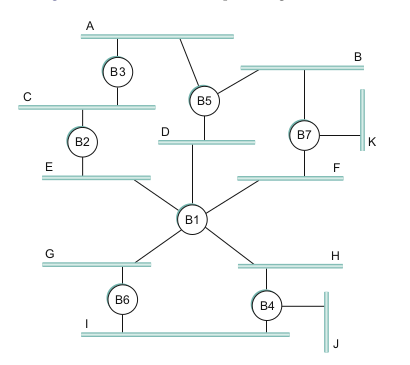
\includegraphics[width=0.5\textwidth
]{images/looped-network.png}
	\caption[Red con un ciclo]{Red con un ciclo}
	\label{fig:looped-network}
\end{figure}

Este problema se resuelve haciendo que los bridges ejecuten un algoritmo de \textbf{spaning tree} distribuido. Se piensa en la LAN extendida como si estuviera representada por un grafo que posiblemente tenga ciclos. Un spanning tree es un subgrafo de este grafo que cubre todos los vértices de la red pero no contiene ciclos. Es decir, un spanning tree mantiene todos los vértices del grafo original pero descarta algunas de las aristas.

El siguiente protocolo es utilizado por un conjunto de bridges para acordar el spanning tree para una LAN extendida en particular y funciona de la siguiente manera: Cada bridge tiene un identificador único; para nuestros propósitos, usamos las etiquetas \(B_1\), \(B_2\), \(B_3\), y así sucesivamente.

Los bridges tienen que intercambiar mensajes de configuración entre sí y luego decidir si son el root o un bridge designado en base a estos mensajes. Específicamente, estos mensajes contienen tres piezas de información:
\begin{enumerate}
  \item El ID del bridge que está enviando el mensaje
  \item El ID del bridge que es considerado el root (hasta el momento)
  \item La distancia, medida en saltos (hops), desde el bridge que envía hasta el root
\end{enumerate}

Inicialmente, cada bridge piensa que es la raíz, y por lo tanto envía un mensaje en cada uno de sus puertos identificándose como la raíz y dando una distancia de 0. 

Al recibir un mensaje sobre un puerto en particular, el bridge verifica si ese nuevo mensaje es mejor que el ya almacenado para ese puerto. Éste se considera mejor que la información actualmente grabada si se cumple alguna de las siguientes condiciones:
\begin{itemize}
  \item Identifica una raíz con un ID más pequeño.
  \item Identifica una raíz con un ID igual pero con una distancia más corta.
  \item El ID de la raíz y la distancia son iguales, pero el bridge que envía tiene un ID más pequeño.
\end{itemize}

Si el nuevo mensaje es mejor que la información actualmente grabada, el bridge descarta la información antigua y guarda la nueva. Sin embargo, primero agrega 1 a la distancia ya que el bridge está a un salto más lejos de la raíz que el bridge que envió el mensaje.

Cuando un bridge recibe un mensaje que indica que no es el bridge raíz, es decir, un mensaje de un bridge con un ID más pequeño, el mismo deja de generar mensajes por su cuenta y en su lugar solo reenvía los de otros bridges, después de agregar 1 al campo de distancia. Del mismo modo, cuando un bridge recibe un mensaje que indica que no es el bridge designado para ese puerto, el bridge deja de generara mensajes sobre ese puerto. Por lo tanto, cuando el sistema se estabiliza, solo el bridge raíz sigue generando mensajes, y los otros bridges están reenviando estos mensajes solo sobre los puertos para los que son el bridge designado. En este punto, se ha construido un spanning tree, y todos los bridges están de acuerdo en qué puertos se utilizan en el mismo. Solo esos puertos pueden usarse para reenviar paquetes de datos en la LAN extendida.

En cierto sentido, es eliminando puertos de la topología que la LAN extendida se reduce a un árbol acíclico. Incluso es posible que un bridge no participe en el reenvío de frames, lo que parece un poco extraño a primera vista. Sin embargo, el algoritmo es dinámico, lo que significa que los bridges siempre están preparados para reconfigurarse en un nuevo spanning tree si algún bridge falla, y por lo tanto, esos puertos y bridges no utilizados proporcionan la capacidad redundante necesaria para recuperarse de fallas.

Una cosa importante a tener en cuenta es que, aunque el algoritmo es capaz de reconfigurar el árbol de expansión cada vez que falla un bridge, no es capaz de reenviar frames por rutas alternativas para evitar un bridge congestionado.

Dado que el objetivo de un bridge es extender una LAN de manera transparente a través de múltiples redes, y dado que la mayoría de las LAN admiten tanto broadcast como multicast, los bridges también deben admitir estas dos características. Broadcast es simple: cada bridge reenvía un frame con una dirección de destino de broadcast en cada puerto activo que no sea el puerto por el que se recibió el frame.

Multicast se puede implementar de la misma manera, con cada host decidiendo por sí mismo si aceptar o no el mensaje.


El algoritmo del árbol de expansión se puede extender para podar las redes sobre las cuales no es necesario reenviar los frames multicast. Cada host que es miembro del grupo M debe periódicamente enviar un frame con la dirección para el grupo M en el campo de origen del encabezado del frame. Este frame tendría como dirección de destino la dirección multicast para los bridges. Sin embargo, esto es ineficiente, por lo que en general se usa la primera opción.

\subsubsection{Limitaciones de los bridges}
En cuanto a la escala, no es realista conectar más de unas pocas LAN mediante bridges. Una razón para esto es que el algoritmo del spanning tree escala linealmente. Una segunda razón es que los bridges reenvían todos los frames de broadcast.

Un enfoque para aumentar la escalabilidad de las LAN extendidas es la VLAN. Las VLAN permiten que una sola LAN extendida se divida en varias LAN separadas. A cada LAN virtual se le asigna un identificador (a veces llamado color), y los paquetes solo pueden viajar de un segmento a otro si ambos segmentos tienen el mismo identificador. Esto tiene el efecto de limitar el número de segmentos en una LAN extendida que recibirá cualquier paquete de broadcast.

En cuanto a la heterogeneidad, los bridges son bastante limitados en los tipos de redes que pueden interconectar. En particular, los bridges utilizan el header del frame de la red y, por lo tanto, solo pueden admitir redes que tengan exactamente el mismo formato para las direcciones. Por lo tanto, los bridges se pueden usar para conectar Ethernets a Ethernets, anillos de tokens a anillos de tokens y una red 802.11 a otra. También es posible poner un bridge entre, por ejemplo, un Ethernet y una red 802.11, ya que ambas redes admiten el mismo formato de dirección de 48 bits. Sin embargo, los bridges no se generalizan fácilmente a otros tipos de redes con diferentes formatos de direccionamiento.

\red{
\section{Nivel Red}
Conmutación y Forwarding. Subredes. Implementación: circuitos virtuales y datagramas. Control de flujo. Concepto de Ruteo. Protocolo IP. Direccionamiento. Broadcasting. Ejemplos de subnetting. Protocolo ARP. Forwarding. ICMP. Traducción de direcciones (NAT).

\section{Ruteo Externo e Interno}
Distance Vector y Link State. Los protocolos RIP y OSPF. Áreas. Inundación confiable.

\section{Nivel de transporte}
Servicios. Primitivas. Protocolos. Servidores de nombres. Manejo de conexión: establecimiento, uso y liberación. Manejo de conexión basados en tiempo. Direccionamiento. Control de flujo. Asignación de buffers. Recuperación de caídas. Multiplexado. Protocolos de nivel 4: Transport Control Protocol (TCP). User Datagram Protocol (UDP) . Mecanismos de control de congestión. Cálculo del RTO. Control de Flujo. Control de errores. Determinación de la performance.

\section*{Congestión}
Introducción al problema de congestión. Curvas de Trafico Enviado vs entregado. Resultado con buffer infinito. Causas de congestión. Control de flujo vs Control de congestión. Taxonomia de Yang y Redan. Soluciones de lazo cerrado y abierto. Concepto de sistemas realimentados. Métricas a sensar para las realimentación. Realimentación implícita y explicita. Determinación de la performance.

\section{Aplicaciones}
Aplicaciones. Correo Electrónico. Protocolos : SMTP, POP3 e IMAP, MIME. Servidores World Wide Web. HTTP. Servidor de Nombres: DNS. Jerarquía de dominios. Resolución de nombres.

\section{Seguridad}
Seguridad en Redes. Marco de Trabajo. Criptografía. Seguridad. Privacidad. Protocolos de Clave Pública y Privada. Algoritmos: DES, 3DES, AES, RSA, MD5 y SHA .Ventajas y desventajas de cada uno. Sus aplicaciones (Autorización, Firma, Confidencialidad e Integridad). Distribución de Claves Públicas. Firewalls. Tunneling. Conceptos de amenazas, ataques, intrusiones.
}
\end{document}

